\chapter{Appendix}
\section{SFR from H$\alpha$ plus 24 \um: procedure and result}
\label{app:halpha}

As mentioned in Section~\ref{sec:data}, we used the H$\alpha$ data from the Nearby Galaxies Survey \citep{Massey07} to create one of our SFR maps. These data cover 10 overlapping fields across the disk of M31 in broad and narrow bands and were observed between August 2000 and September 2002; we obtained them  from the NOAO Science Archive. Making a spatially resolved SFR map of M31 using H$\alpha$ emission requires removal of background and stellar emission in each field, masking out foreground stars and saturated regions, creating a mosaic of H$\alpha$ continuum-subtracted images, and finally correcting for the flux contribution to the \halpha filter from the [N II] 6583~\AA\ line.

The Nearby Galaxies survey $R$-band images were used to remove the stellar emission from H$\alpha$ using the scaling factor between fluxes in these two band passes determined by \citet{Azimlu11}. They estimated continuum emission in each H$\alpha$ image, using photometric measurements in both \halpha and R-band images, and determined the scaling factor. These images were observed from a ground-based telescope over two years' time. Consequently, there is a non-negligible sky contribution in the background which must be estimated and removed from each image in both bands. Unfortunately, there is no nearby `blank-sky' image taken with the same instrument available from which to measure the sky contribution, which makes the removal of background emission even harder. The only remaining choice is to subtract the local background for each region. However, subtracting local backgrounds from each image will result in a non-smooth background in the final mosaic image. 


\begin{figure*}
\centering
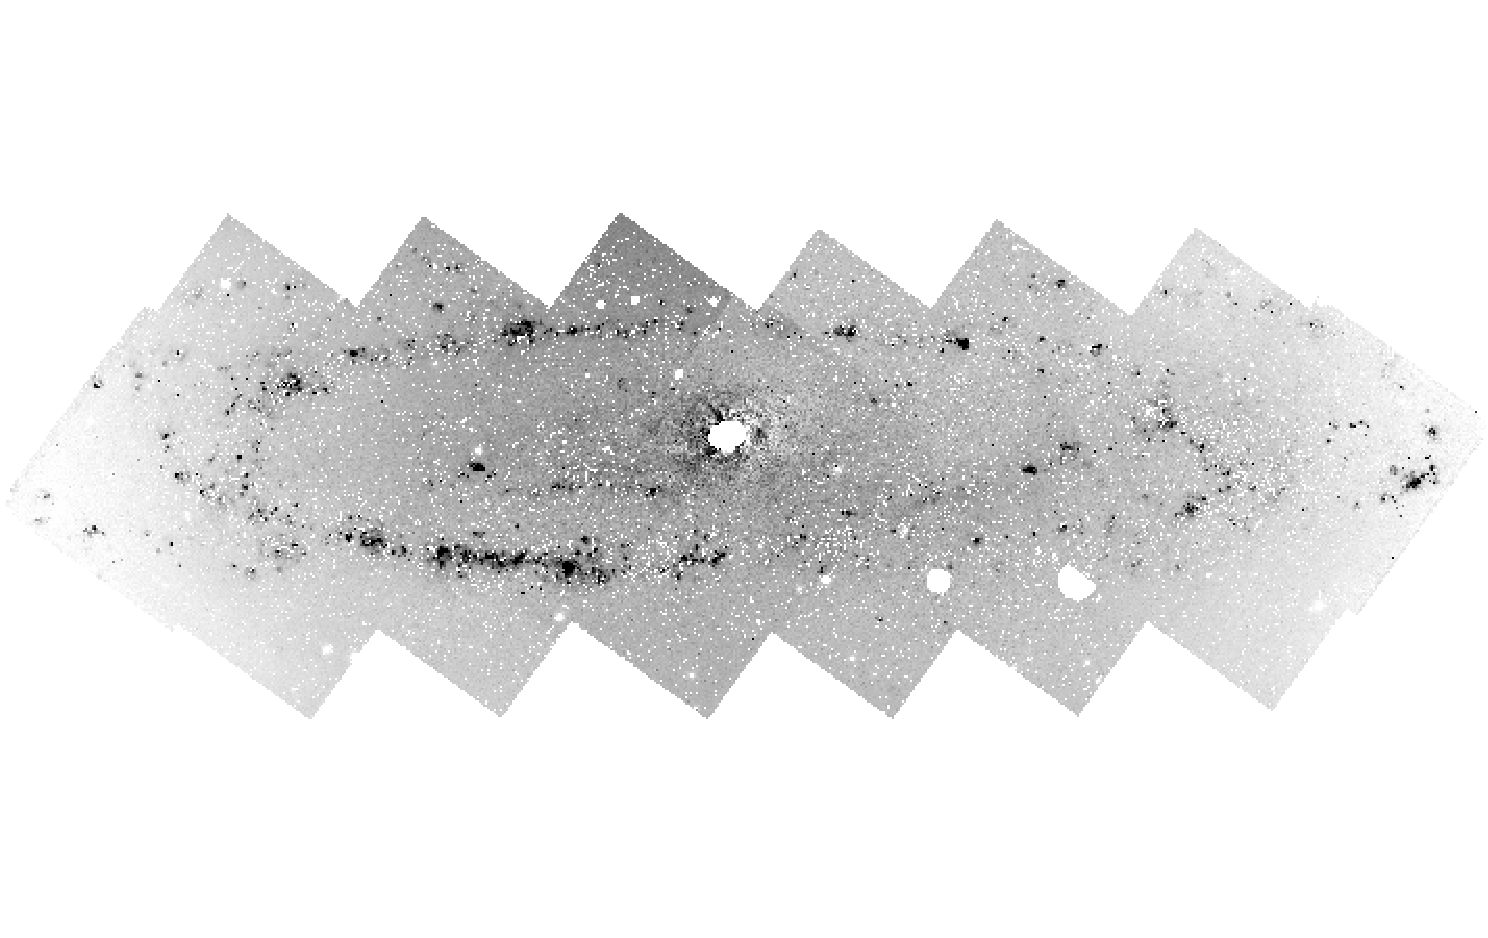
\includegraphics[width=164mm]{../image_paper1/halpha.pdf}
\caption{Mosaic created using the Montage programme from six fields of H$\alpha$ emission images of M31 from \citet{Massey07}. The resulting image from Montage was continuum-subtracted and masked for all point sources. The centre of the galaxy was masked out due to saturation of data in the continuum $R$-band image.}
\label{fig:halpha}
\end{figure*}

To create the final mosaic, first we removed the background from each region in both the \halpha and $R$-band images. The second step was to subtract the continuum from the \halpha images. Since both \halpha and $R$-band images were aligned on the same coordinate grid, for each field, the R-band image multiplied by the scaling factor was subtracted from each corresponding \halpha image. At the end, we masked out all the foreground and saturated regions which include a $10\arcmin \times 10\arcmin$ region in the centre of the galaxy. To account for the flux contribution of the [N II] emission we used the flux ratio ${\rm [NII]}/{\rm H}\alpha = 0.54$ from \citet{Kennicutt08}, and subtracted it from the \halpha map. We created the final mosaic image, Figure~\ref{fig:halpha}, using the Montage program \citep{Berriman08}.

Creating the SFR map using \halpha plus 24 \um was described in Section~\ref{sec:sfr_halpha}. In order to investigate the SFR laws, we used the same method of the fitting as Section~\ref{sec:fitting}. The fitting results using SFR(\halpha $+$ 24~\um) are more or less the same as the other two SFR tracers. The main reason for this difference is the missing data in the centre of the galaxy and the lack of smooth background in the \halpha data. Thus we did not include the SFR(\halpha $+$ 24 \um) in our final analysis.

\newpage
\section{More results from the fitting of the extended Schmidt law}
\label{app:es,figs}
Section~\ref{sec: sfl} discusses testing the extended Schmidt law and shows results for one SFR/gas tracer combination. Here we present the plots for the remaining SFR/gas tracer combinations.


\begin{figure*}
    \centering
    \begin{subfigure}[b]{0.5\textwidth}
        \centering
        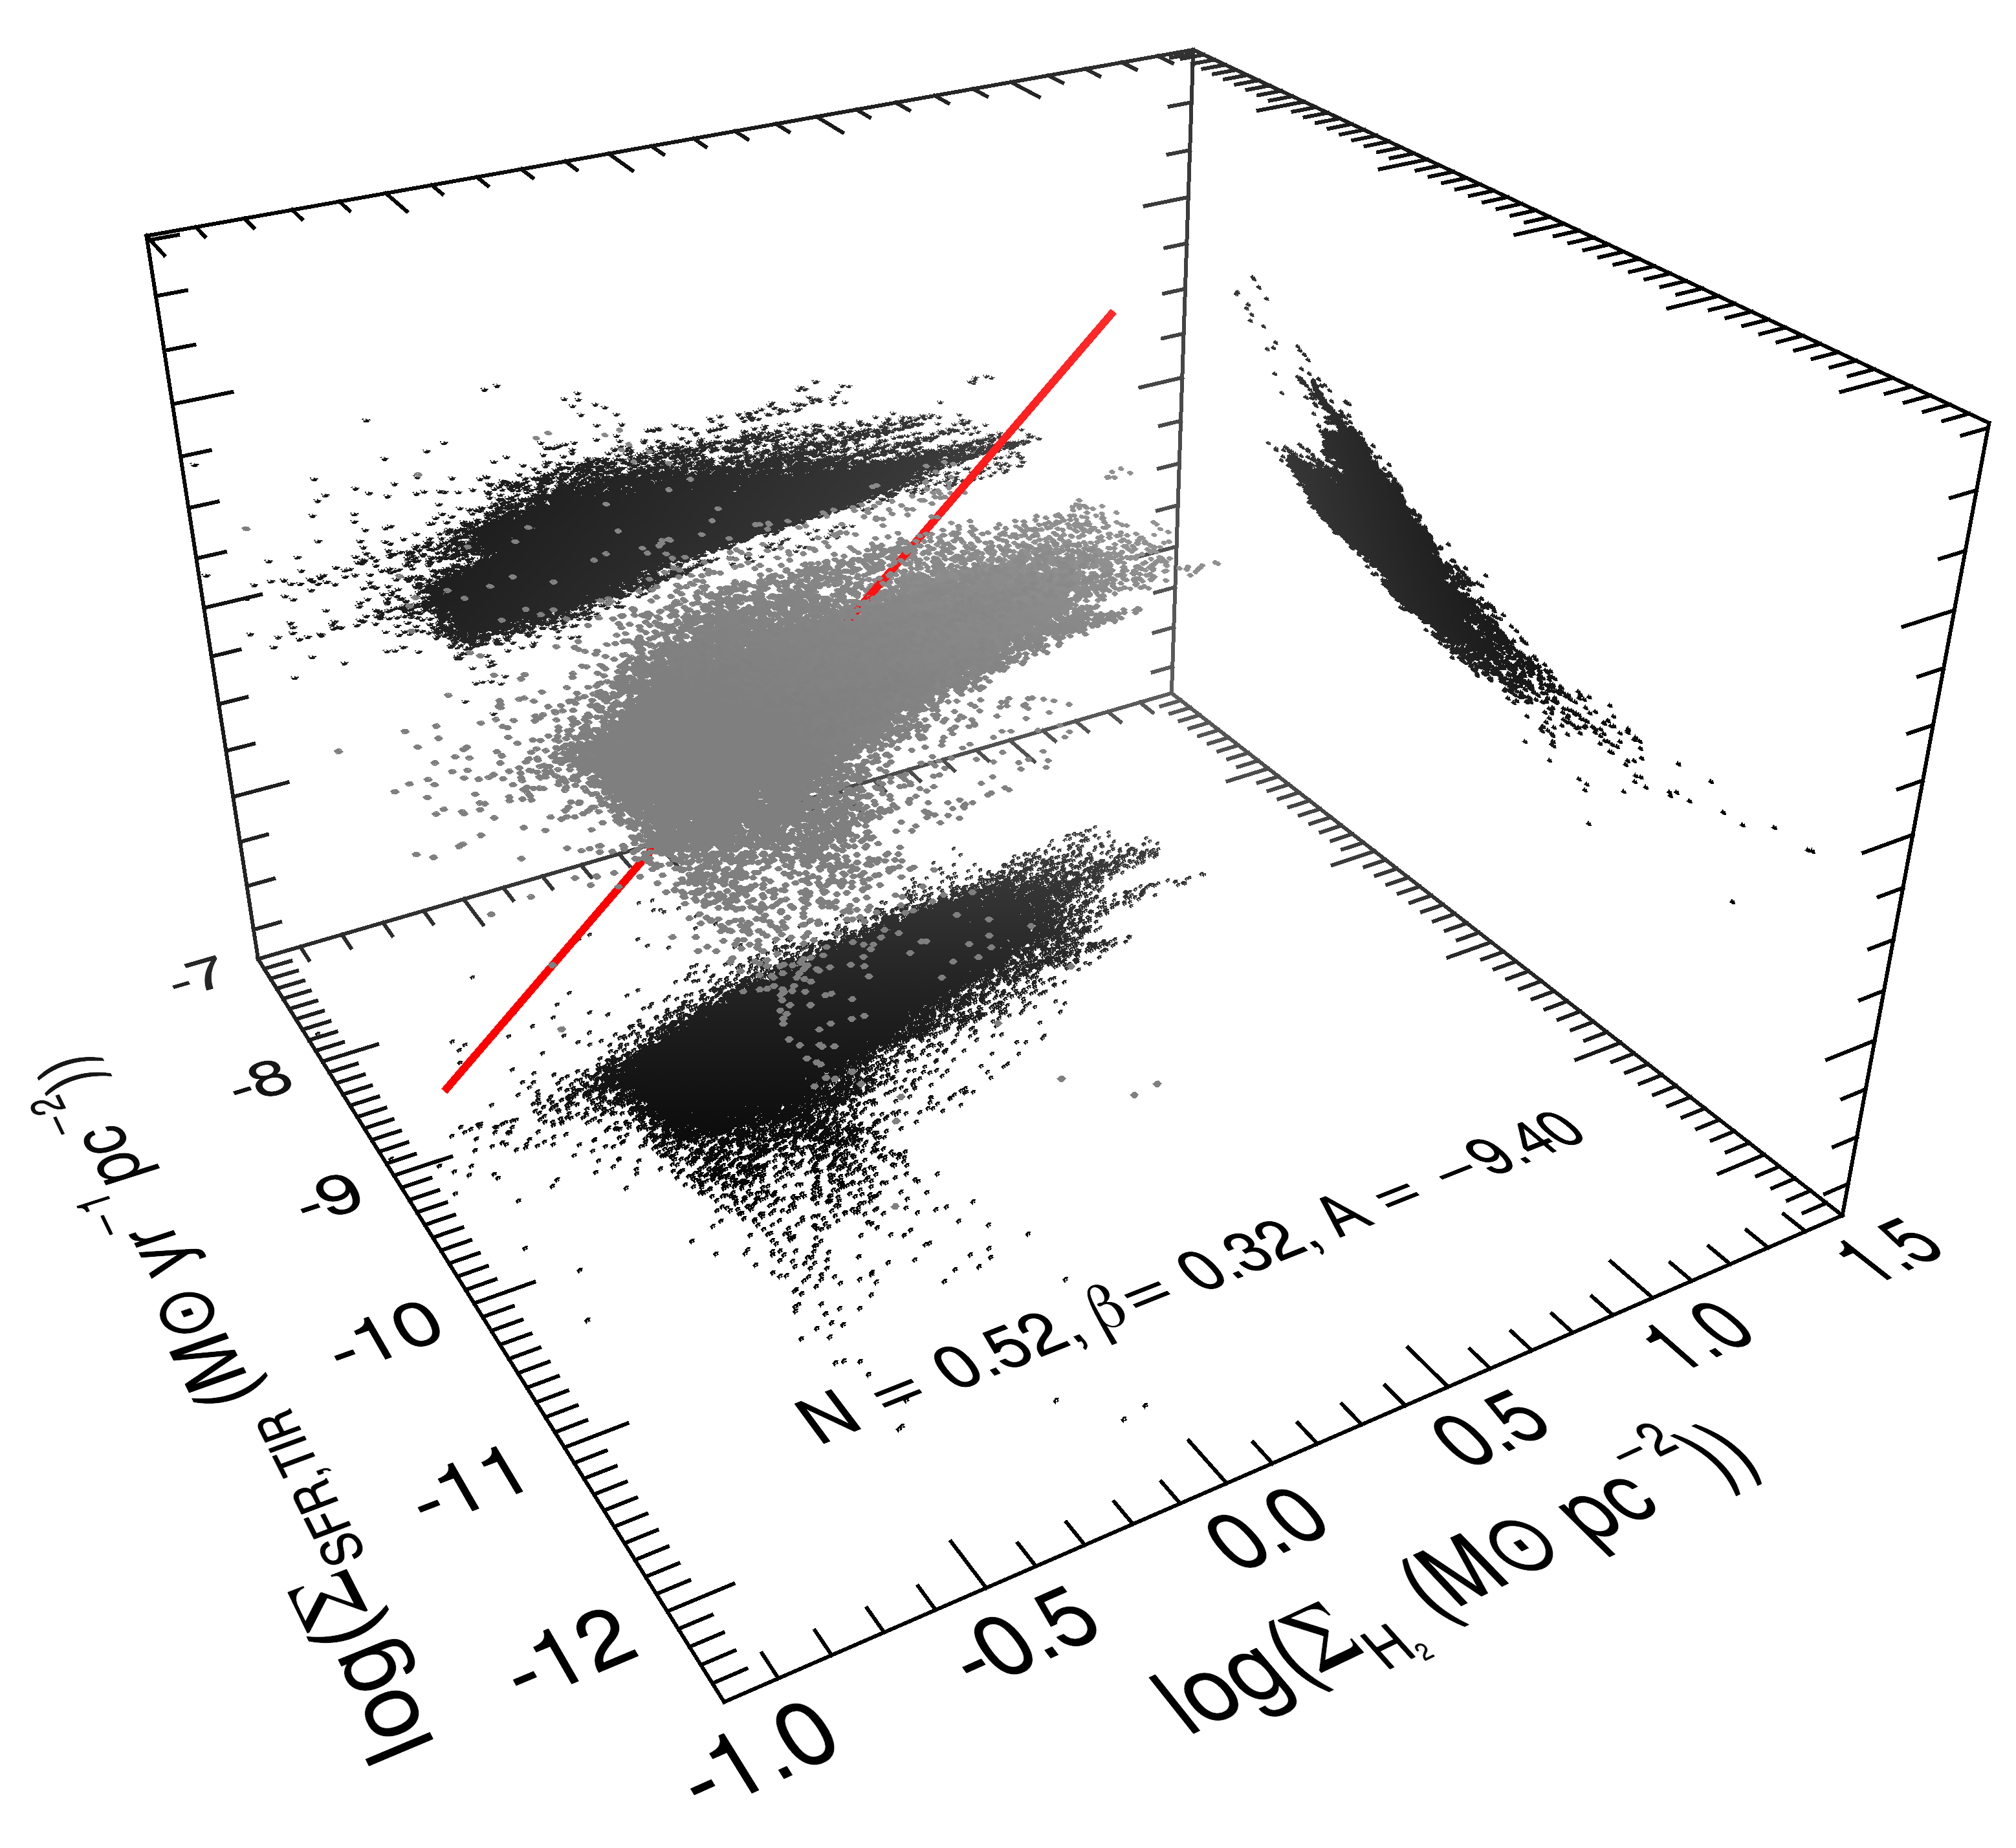
\includegraphics[width=\textwidth]{../image_paper1/es_tot_fir_vs_h2.png}
        \caption{Surface density of SFR(TIR) vs surface density of H$_2$ and surface density of stellar mass ($z$-axis) }
        \label{fig:es,all,fir,h2}
    \end{subfigure}
    \hfill
    \begin{subfigure}[b]{0.5\textwidth}
        \centering
        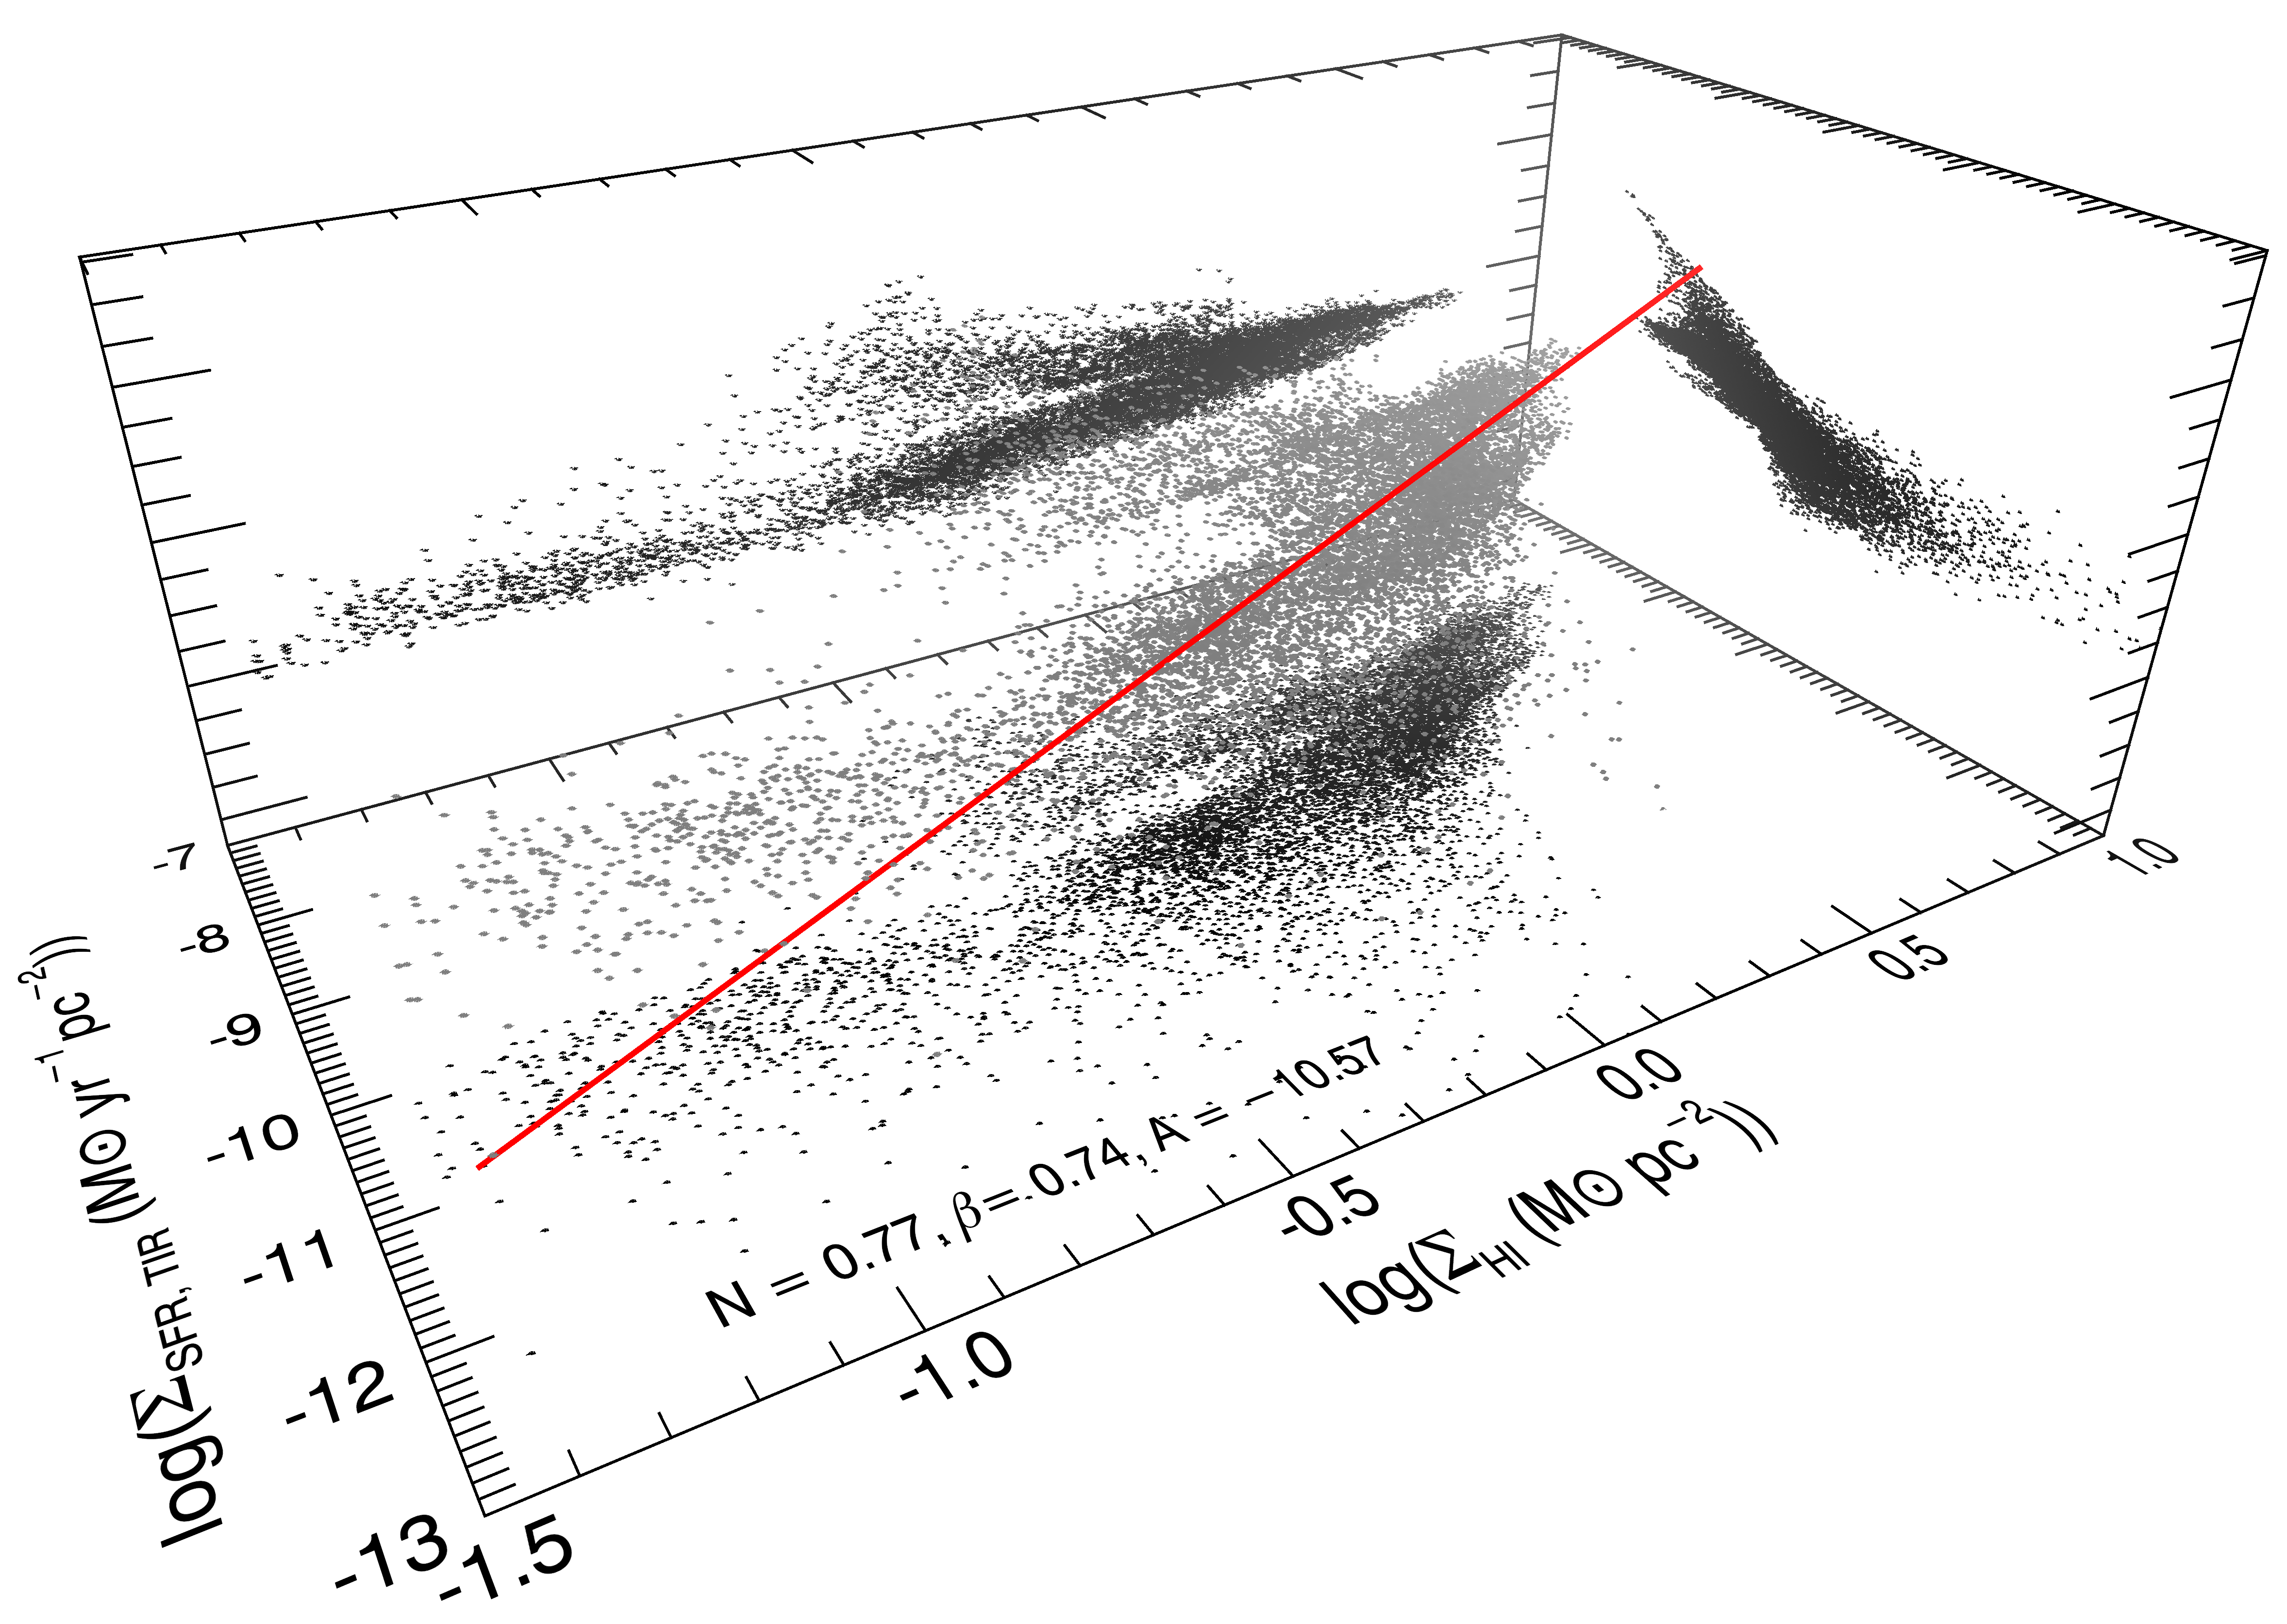
\includegraphics[width=\textwidth]{../image_paper1/es_tot_fir_vs_hi2.png}
        \caption{Surface density of SFR(TIR) vs surface density of H\,{\sc I} and surface density of stellar mass ($z$-axis) }
        \label{fig:es,all,fir,hi}
    \end{subfigure}
    \hfill
   \begin{subfigure}[b]{0.5\textwidth}
        \centering
        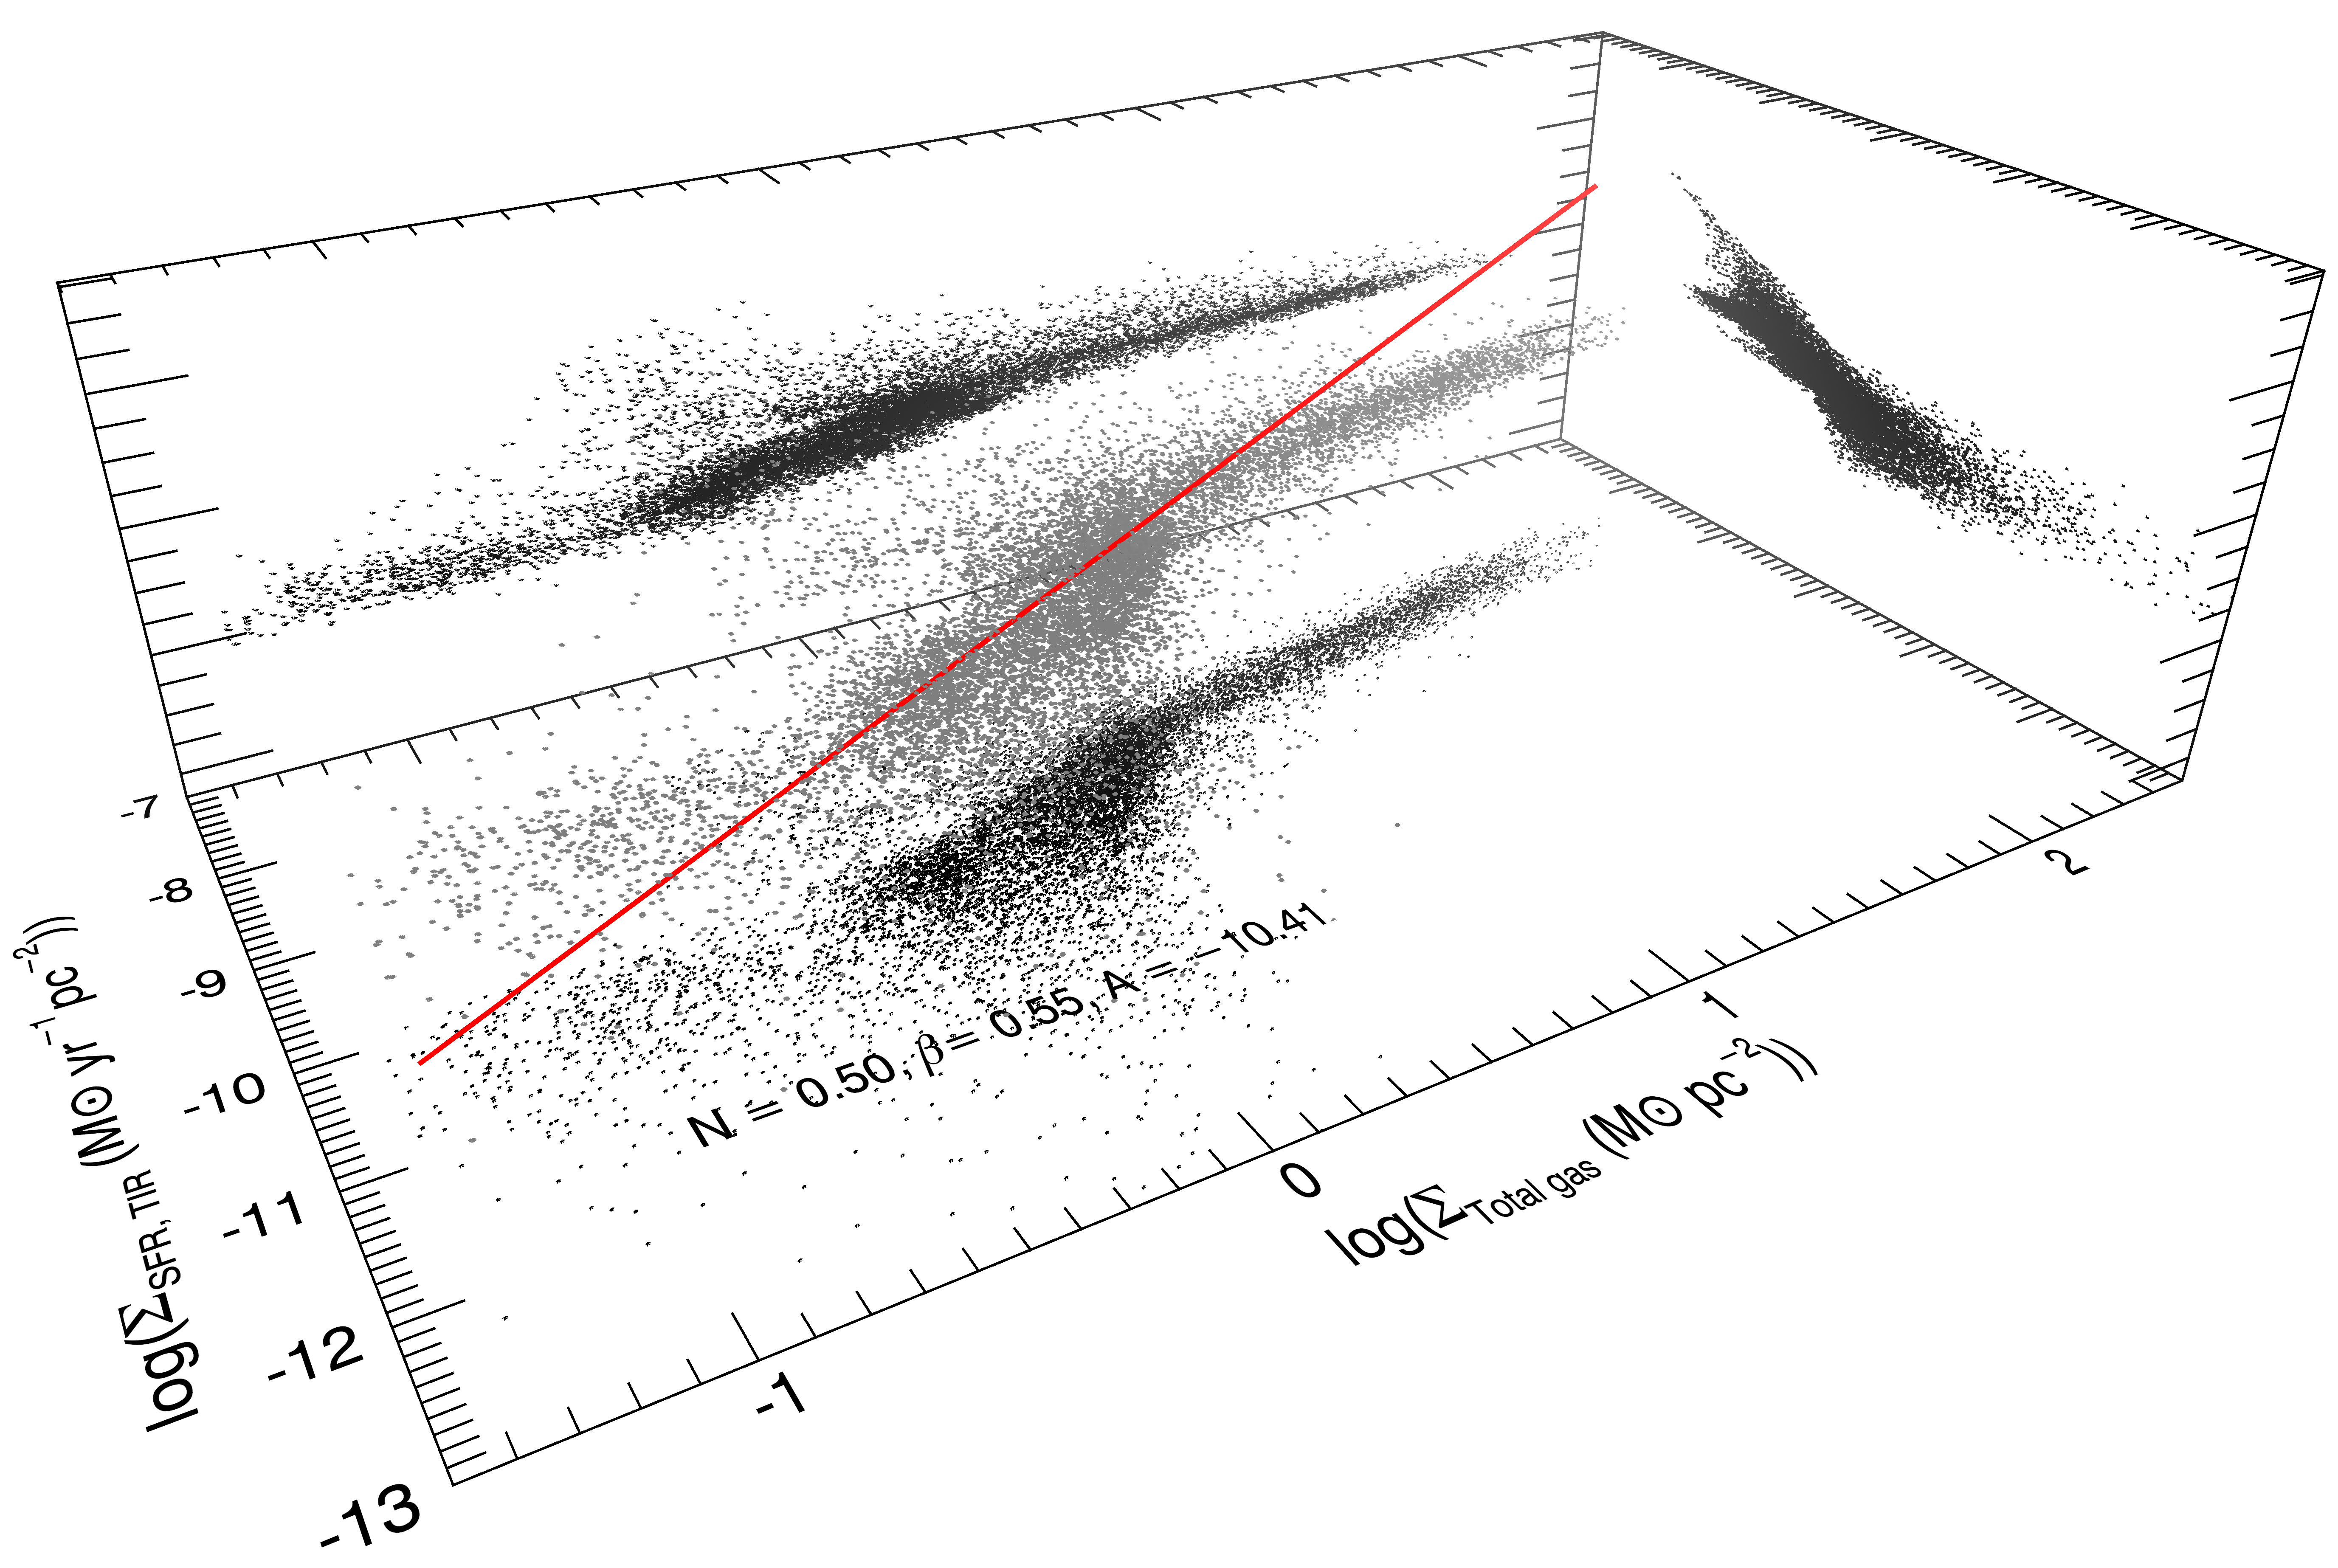
\includegraphics[width=\textwidth]{../image_paper1/es_tot_fir_vs_tot2_f.png}
        \caption{Surface density of SFR(TIR) vs surface density of total gas and surface density of stellar mass ($z$-axis)}
        \label{fig:es,all,fir,tot}
    \end{subfigure}
       \caption{Same as Figure~\ref{fig:es,all,fuv,tot}. Here, from top to bottom plots show the surface density of the SFR(TIR) vs. surface density of H$_2$, surface density of H\,{\sc I}, and the surface density of total gas, respectively. As in Figure~\ref{fig:ks_all}, the analyses use different pixel sizes: each point in the plots with the surface density of H$_2$ as a tracer of gas mass represents a region of size $\sim$30~pc and each point in the plots with the surface density of H\,{\sc I} or total gas mass represents a region of size $\sim$155~pc. Solid lines show the best fit, using the mean value of the ranges in Table~\ref{table:res}.}
       \label{fig:es,fir}
\end{figure*}


\begin{figure*}
    \centering
     \begin{subfigure}[b]{0.5\textwidth}
        \centering
        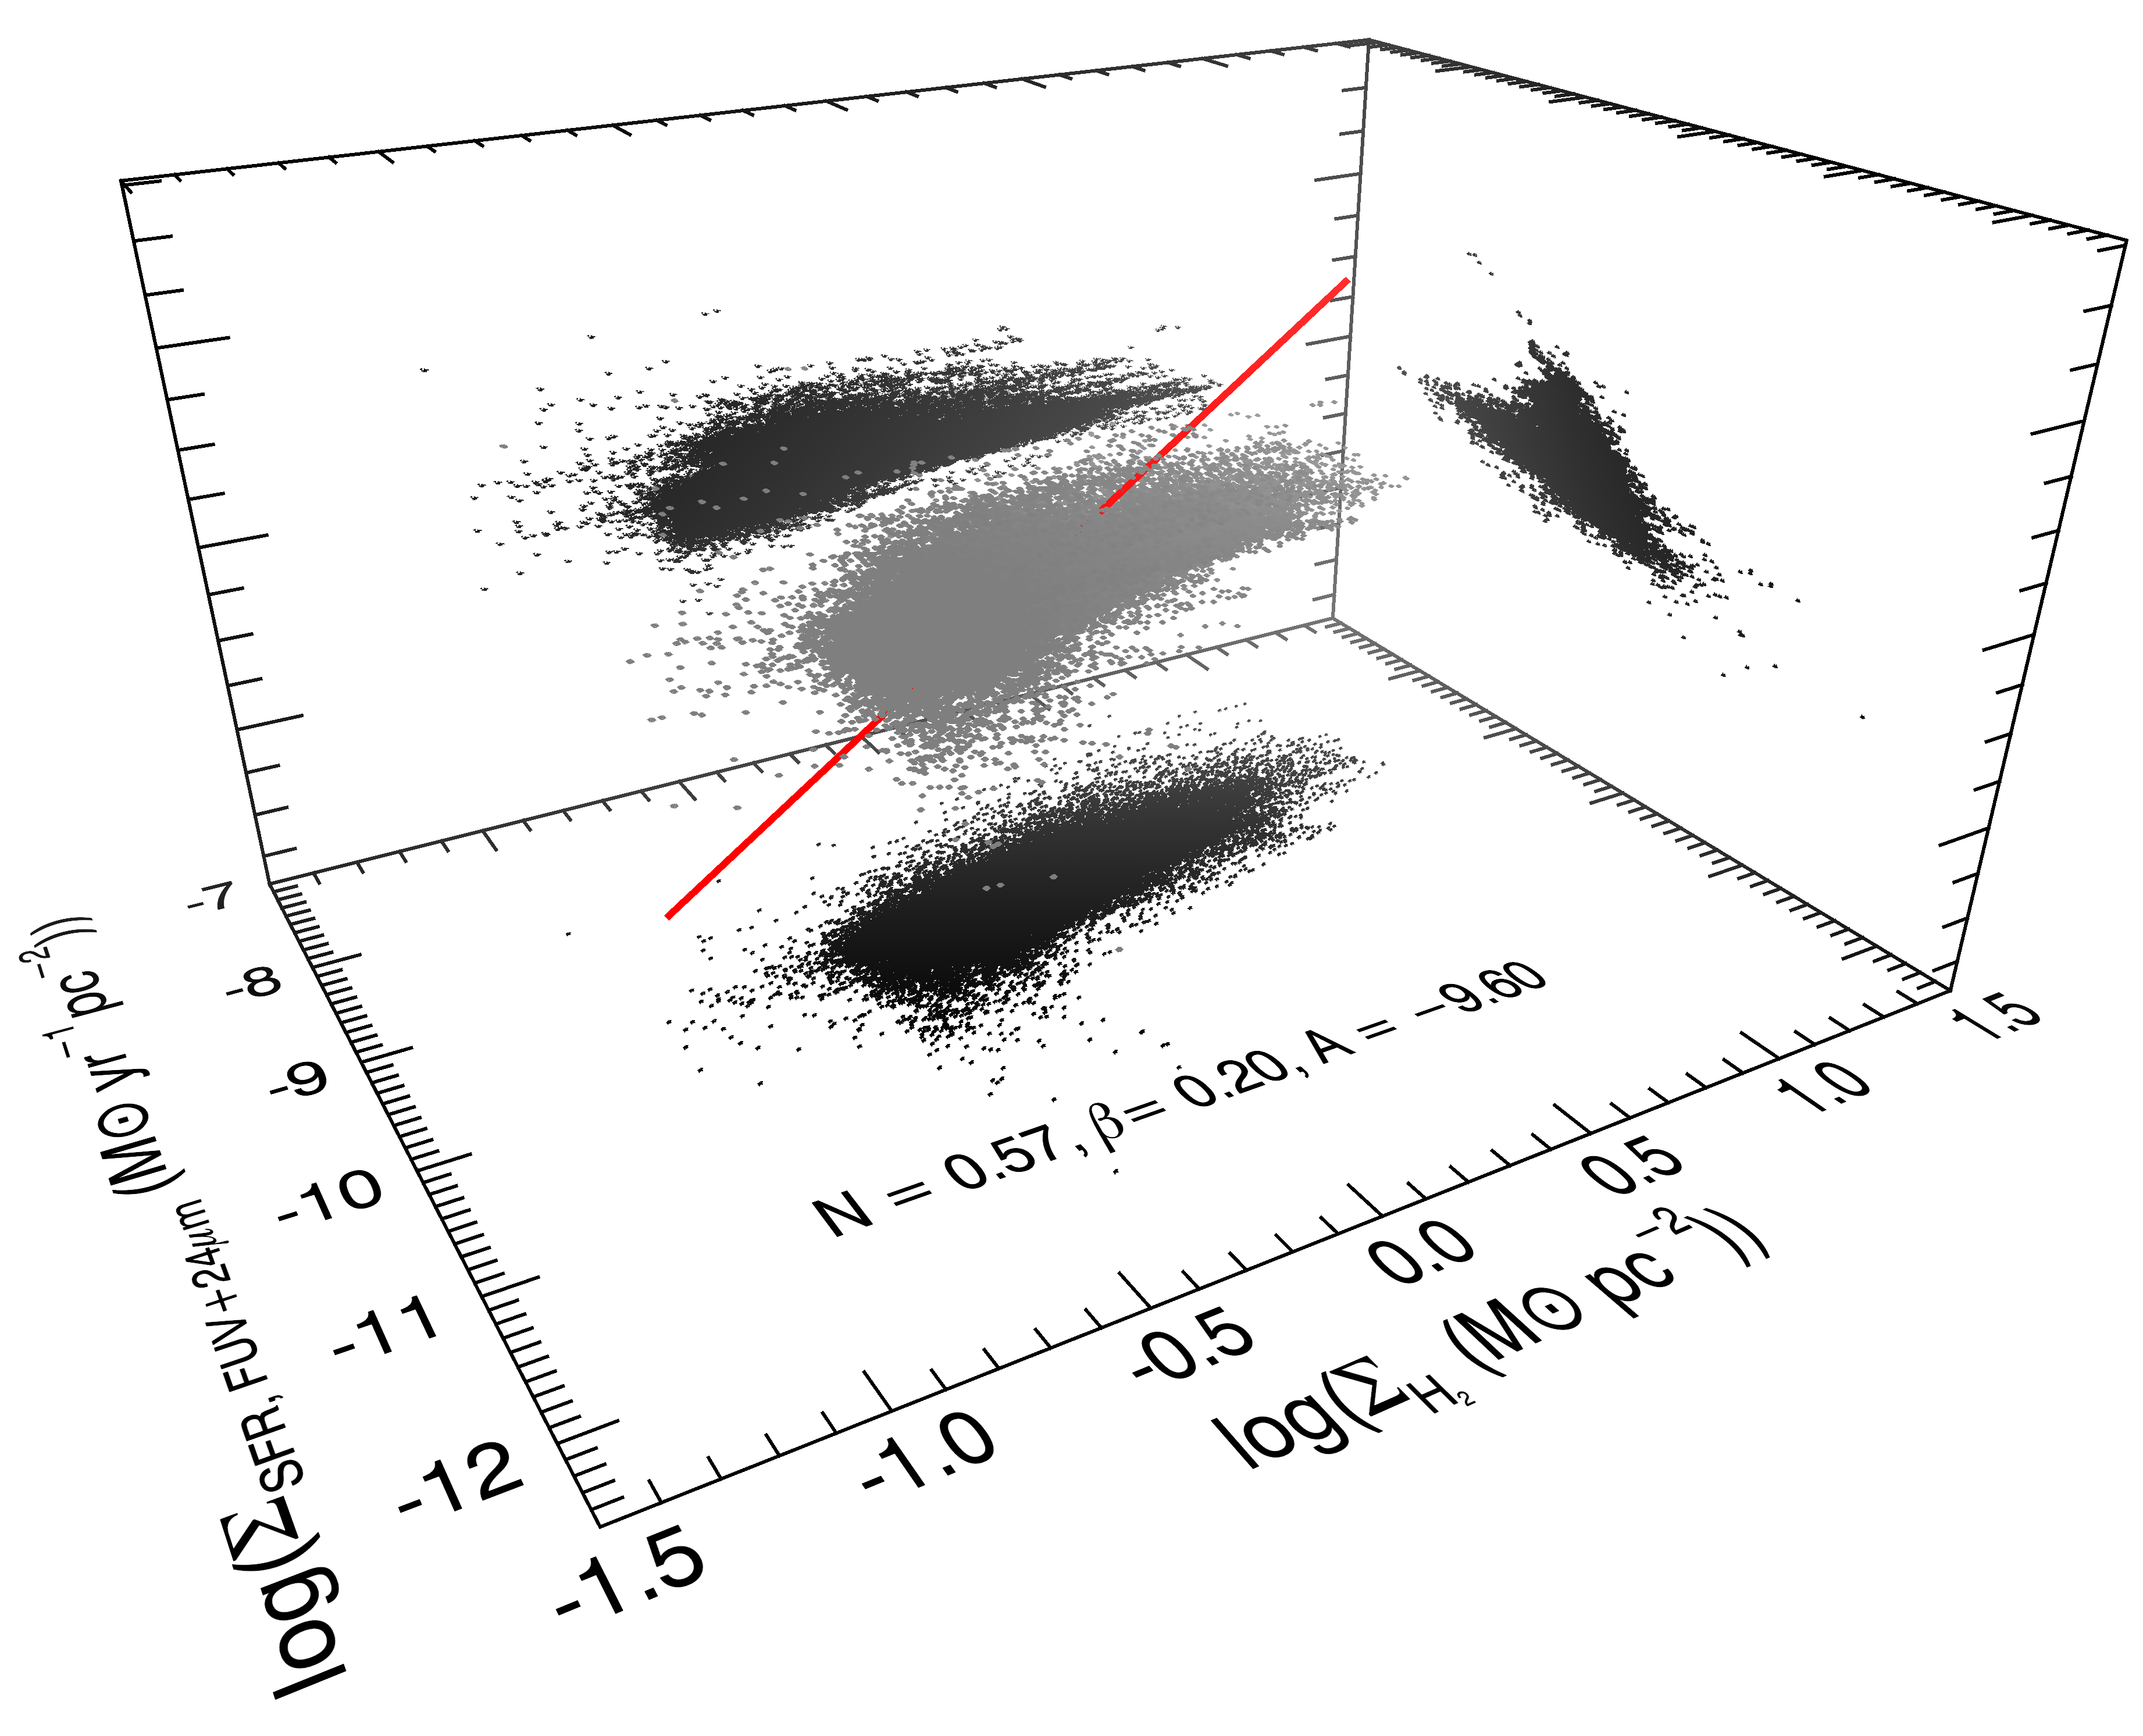
\includegraphics[width=\textwidth]{../image_paper1/es_tot_fuv_vs_h22_f.png}
        \caption{Surface density of SFR(FUV+24~$\mu$m) vs surface density of H$_2$ and surface density of stellar mass ($z$-axis)}
        \label{fig:es,all,fuv,h2}
    \end{subfigure}
     \hfill
   \begin{subfigure}[b]{0.5\textwidth}
        \centering
        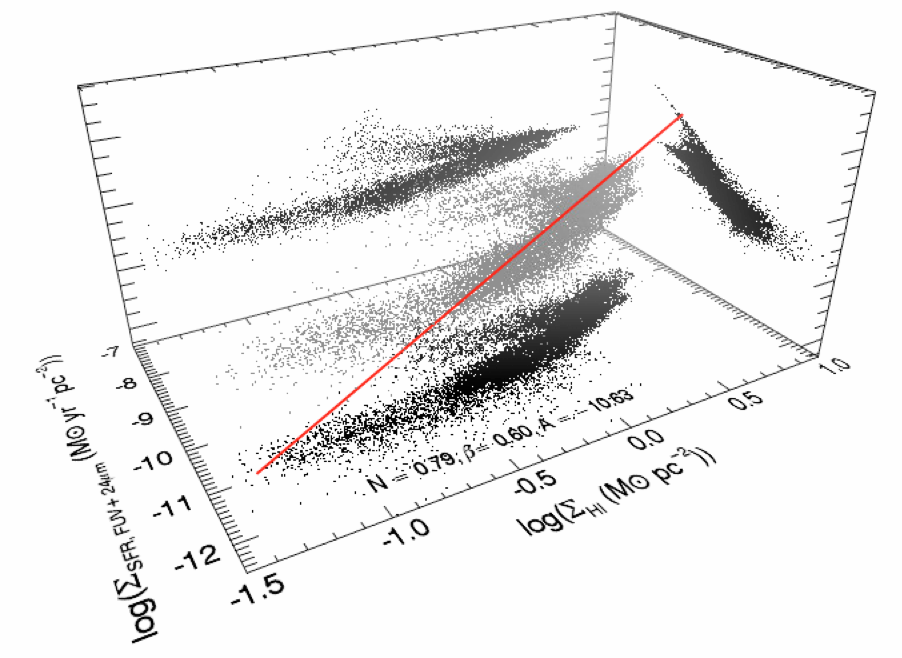
\includegraphics[width=\textwidth]{../image_paper1/es_tot_fuv_vs_hi2.png}
        \caption{Surface density of SFR(FUV+24~$\mu$m) vs surface density of H\,{\sc I} and surface density of stellar mass ($z$-axis)}
        \label{fig:es,all,fuv,hi}
    \end{subfigure}
   \caption{Same as Figure~\ref{fig:es,fir}, but in this figure we used FUV + 24~$\mu$m as a tracer of the SFR. The plot of the surface density of the SFR(FUV+24~$\mu$m) vs the surface density of the total gas is shown in Figure~\ref{fig:es,all,fuv,tot} in the main text.}
\end{figure*}

         
\begin{figure*}
  \centering
   \begin{subfigure}[b]{0.5\textwidth}
        \centering
        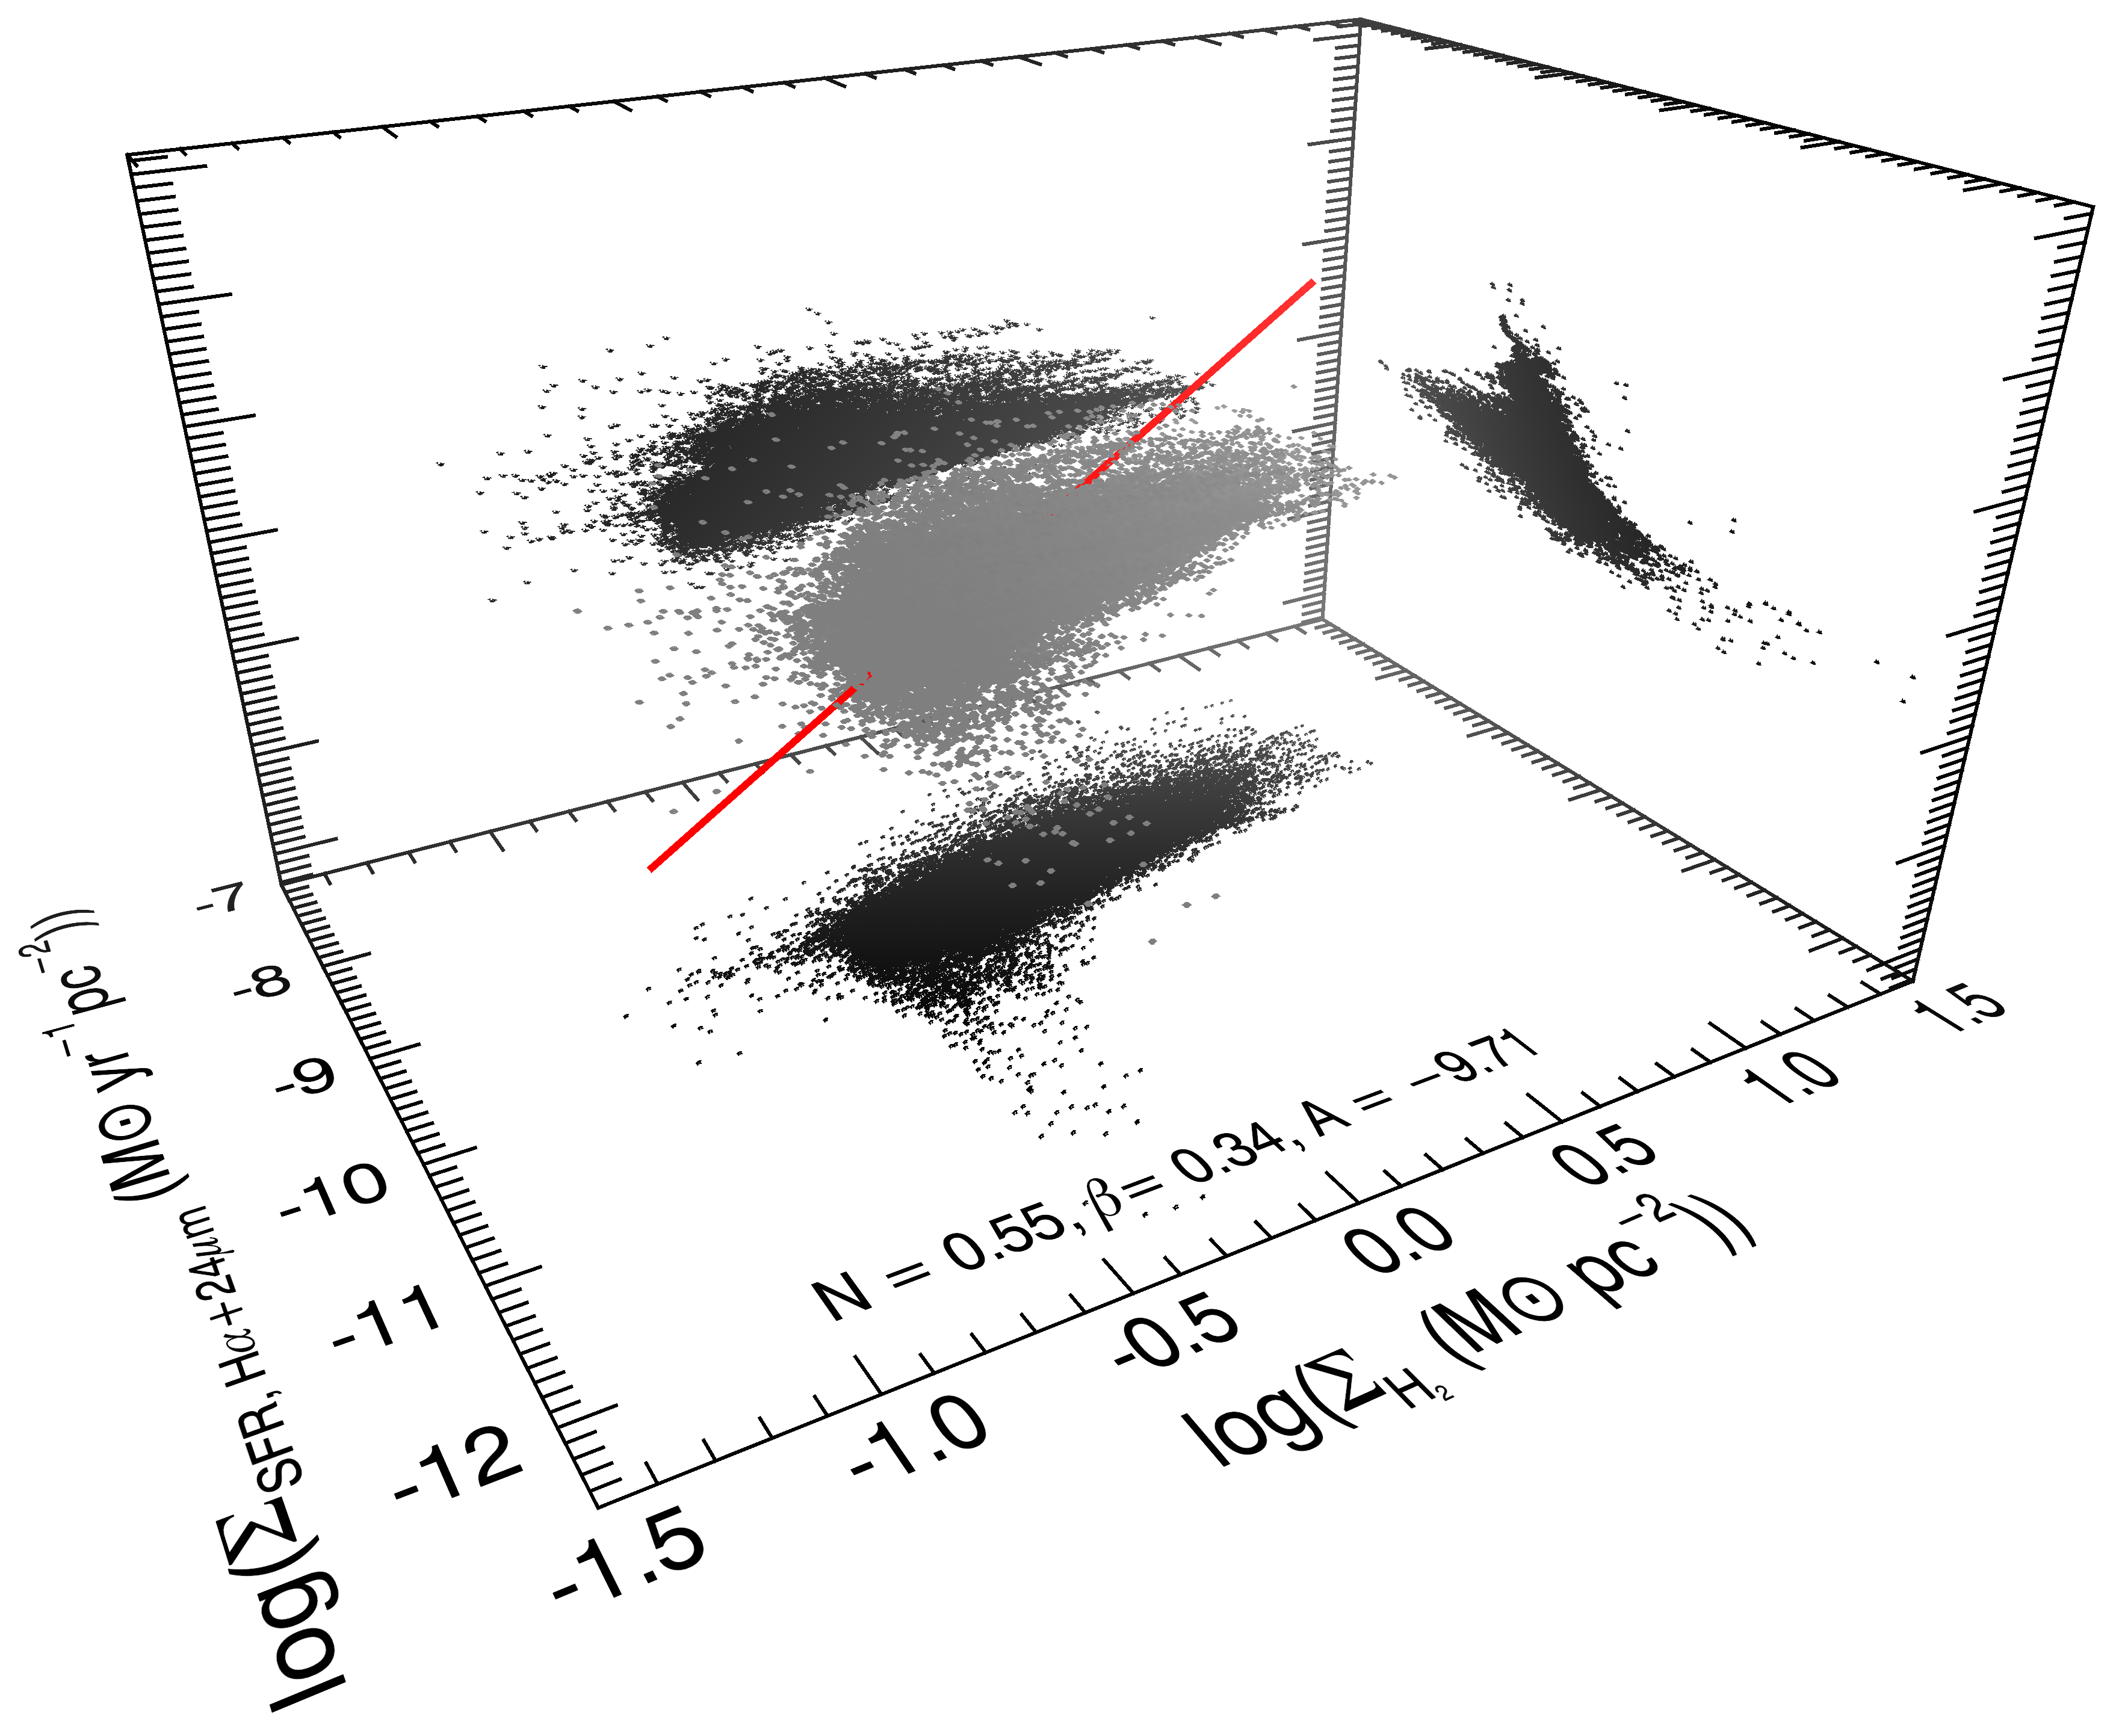
\includegraphics[width=\textwidth]{../image_paper1/es_tot_halpha_vs_h22_f.png}
        \caption{Surface density of SFR(H$\alpha$+24~$\mu$m) vs surface density of H$_2$ and surface density of stellar mass ($z$-axis)}
        \label{fig:es,all,halpha,h2}
    \end{subfigure}
     \hfill
      \begin{subfigure}[b]{0.5\textwidth}
        \centering
        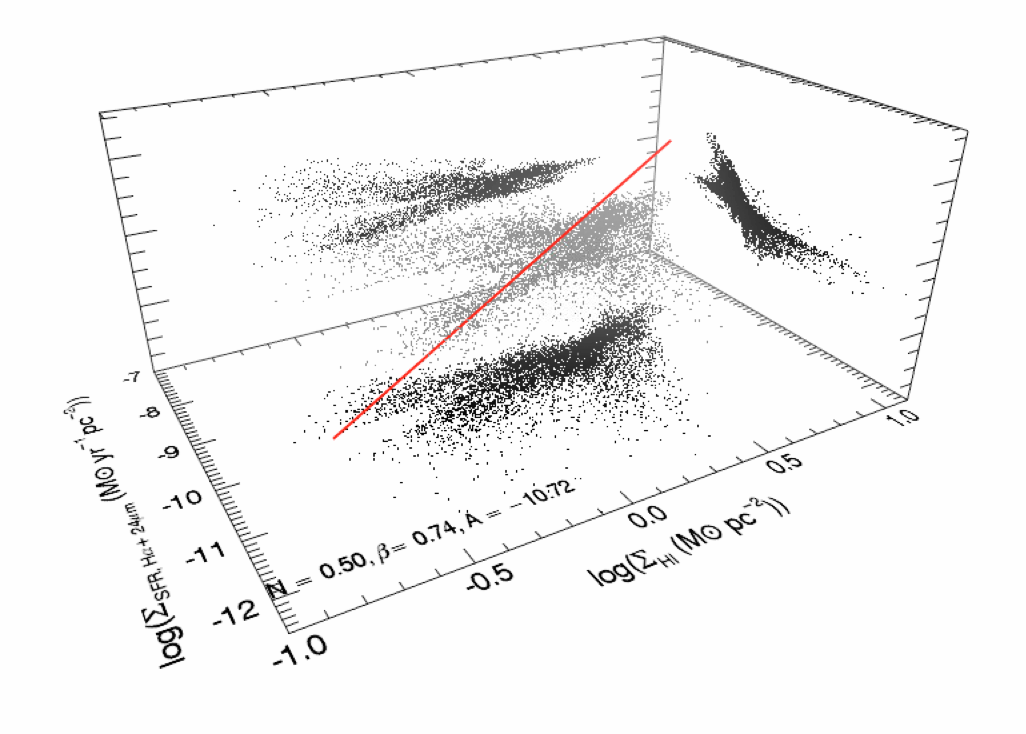
\includegraphics[width=\textwidth]{../image_paper1/es_tot_halpha_vs_hi2.png}
        \caption{Surface density of SFR(H$\alpha$+24~$\mu$m) vs surface density of H\,{\sc I} and surface density of stellar mass ($z$-axis)}
        \label{fig:es,all,halpha,hi}
    \end{subfigure}
    \hfill
    \begin{subfigure}[b]{0.5\textwidth}
        \centering
        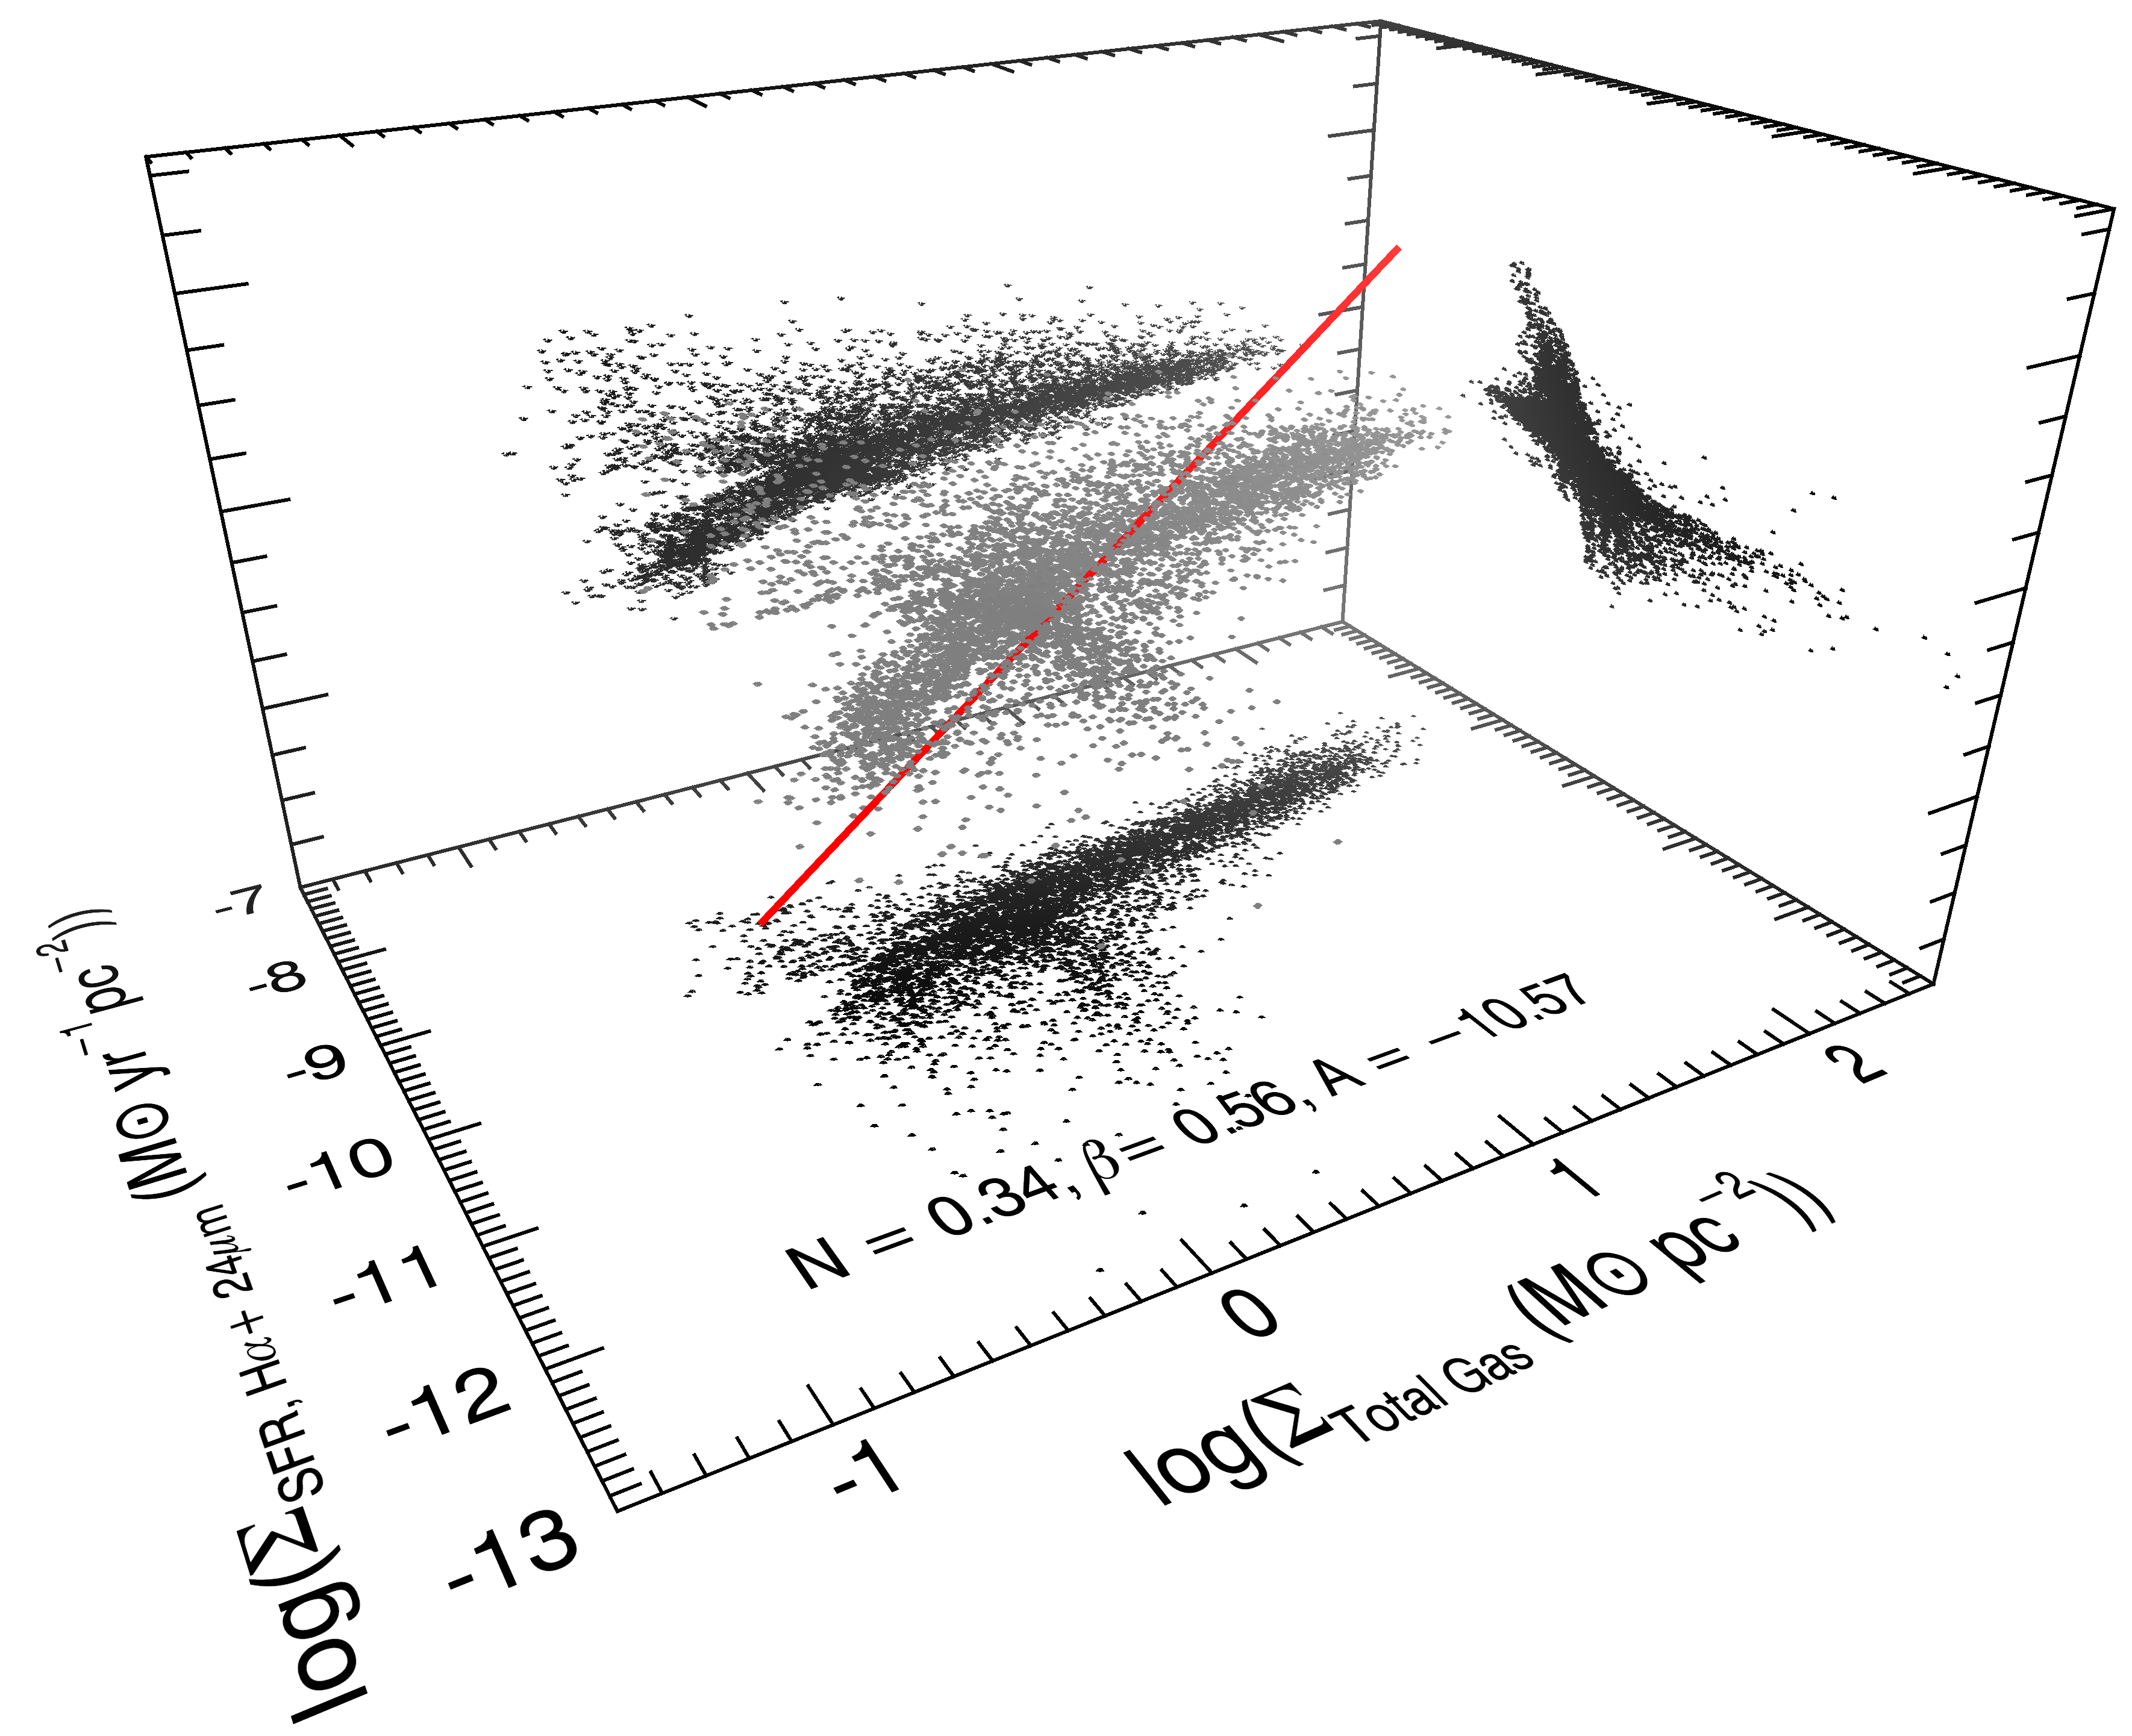
\includegraphics[width=\textwidth]{../image_paper1/es_tot_halpha_vs_tot2_f.png}
        \caption{Surface density of SFR(H$\alpha$+24~$\mu$m) vs. surface density of total gas and surface density of stellar mass ($z$-axis)}
        \label{fig:es,all,halpha,tot}
    \end{subfigure}
    \caption{Same as Figure~\ref{fig:es,fir}, but in this figure we used H$\alpha$ + 24~$\mu$m as a tracer of the SFR.}
\end{figure*}


\section{Results of training for one-dimensional self-organizing maps}
\label{app: high_Z_1d_soms}
As mentioned in Sec.~\ref{sec: 1D}, we changed the size of the SOM from $1\times2$ to $1\times22$. In that section we show some example of the results, here we show the rest of the maps to monitor the changes in the map in various sizes.

\label{app: 1d}
    \begin{figure}
        \begin{subfigure}[b]{0.5\textwidth}
            \centering
            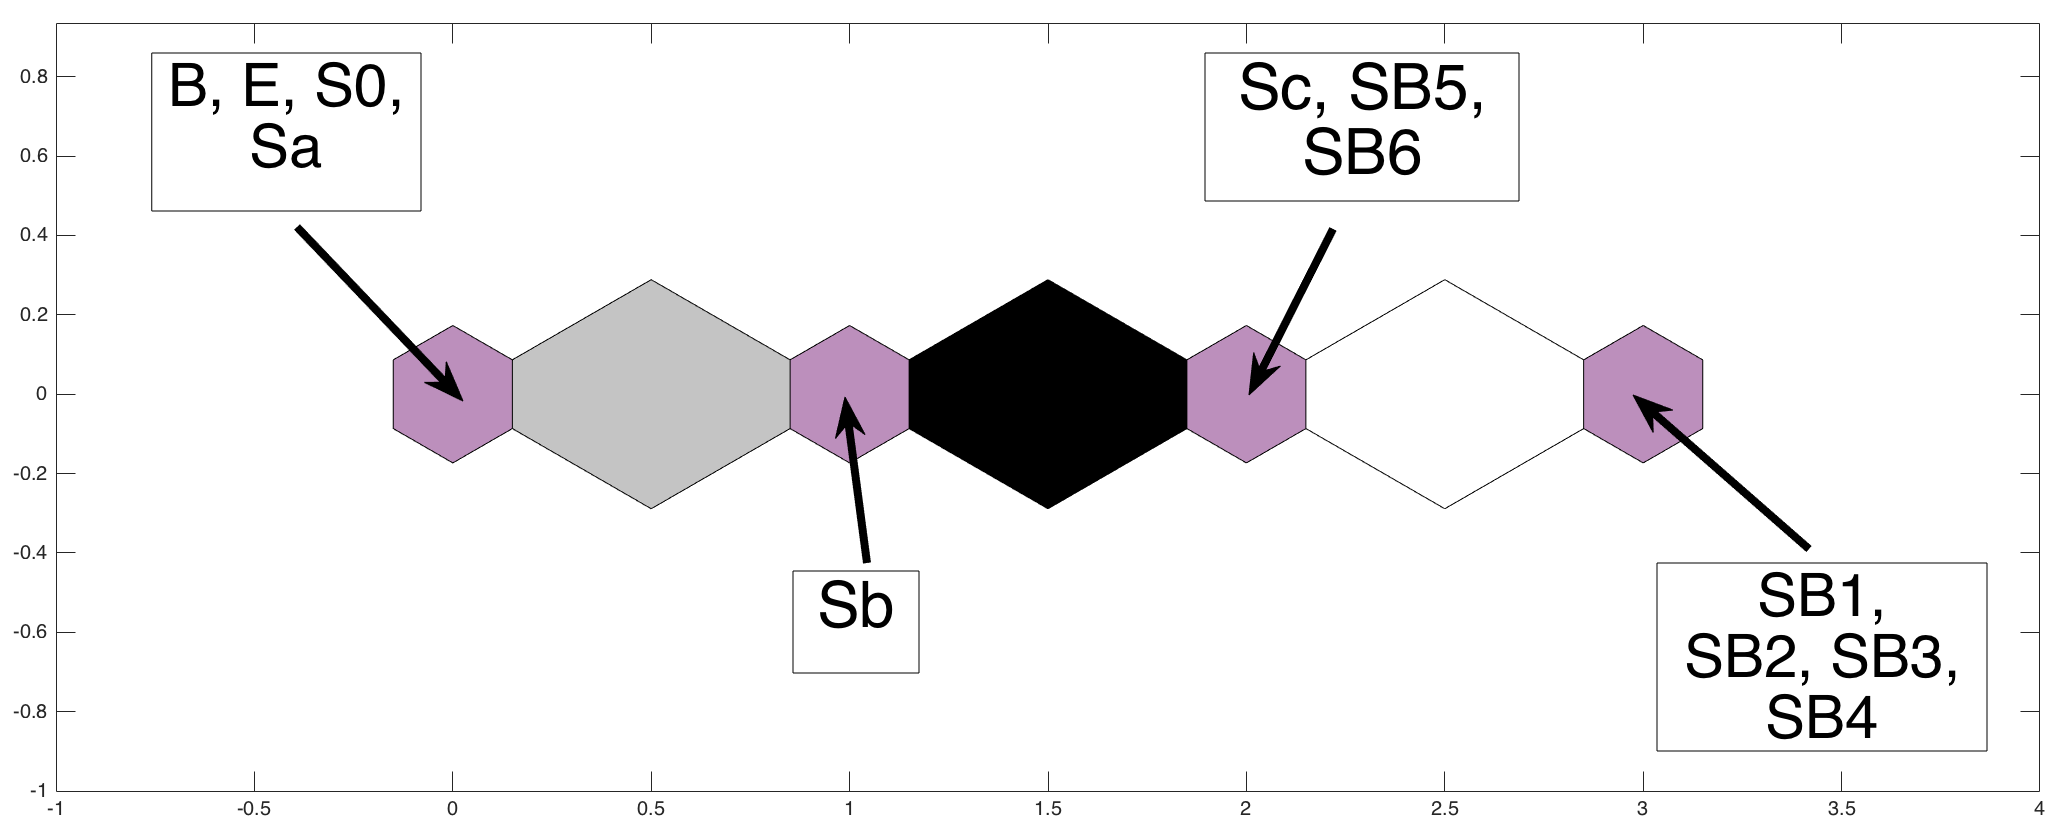
\includegraphics[width=\textwidth]{../image_paper2/1d/apps/dist_1_by_4.png}
            %\caption{$1\times4$ weight map}
             %\label{fig: 1by4T}
        \end{subfigure}
        \hfill
        \begin{subfigure}[b]{0.5\textwidth}
             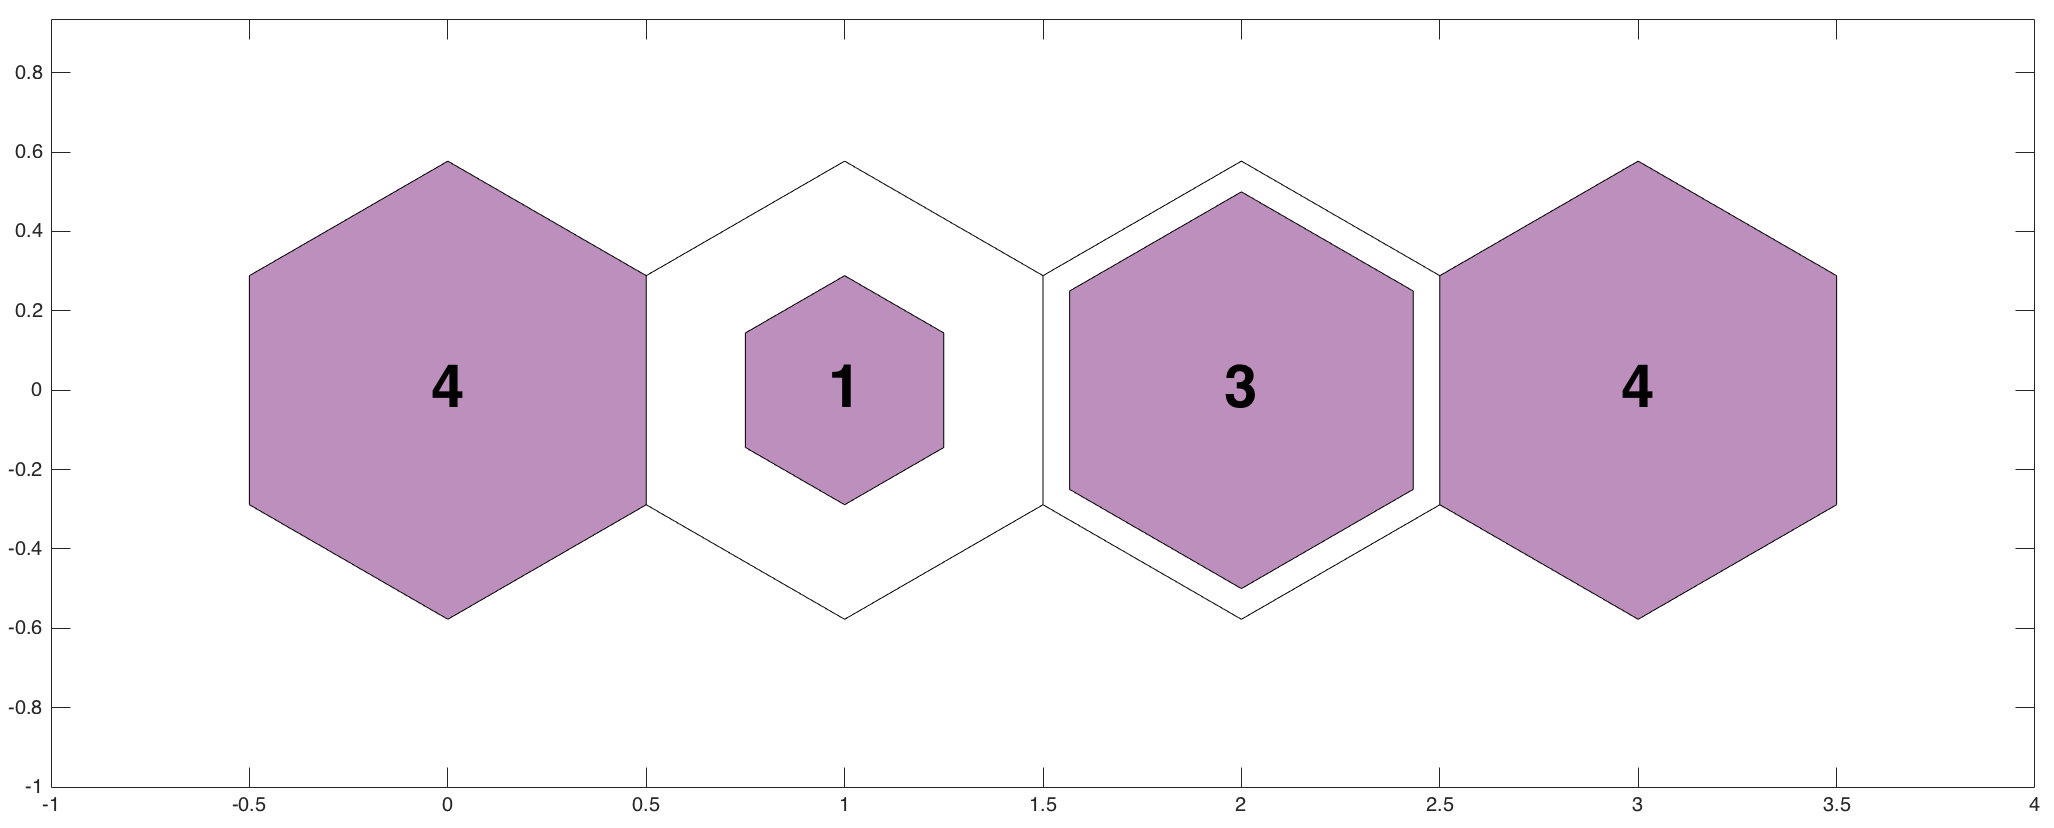
\includegraphics[width=\textwidth]{../image_paper2/1d/apps/hit_t_1_by_4.png}
             %\caption{$1\times4$ hits map}
             %\label{fig: 1by4Thits}
        \end{subfigure}
                \caption{Results of training network in $1\times4$~grid.}
         \label{fig: 1by4T}
    \end{figure}
    
    \begin{figure}
        \begin{subfigure}[b]{0.5\textwidth}
            \centering
            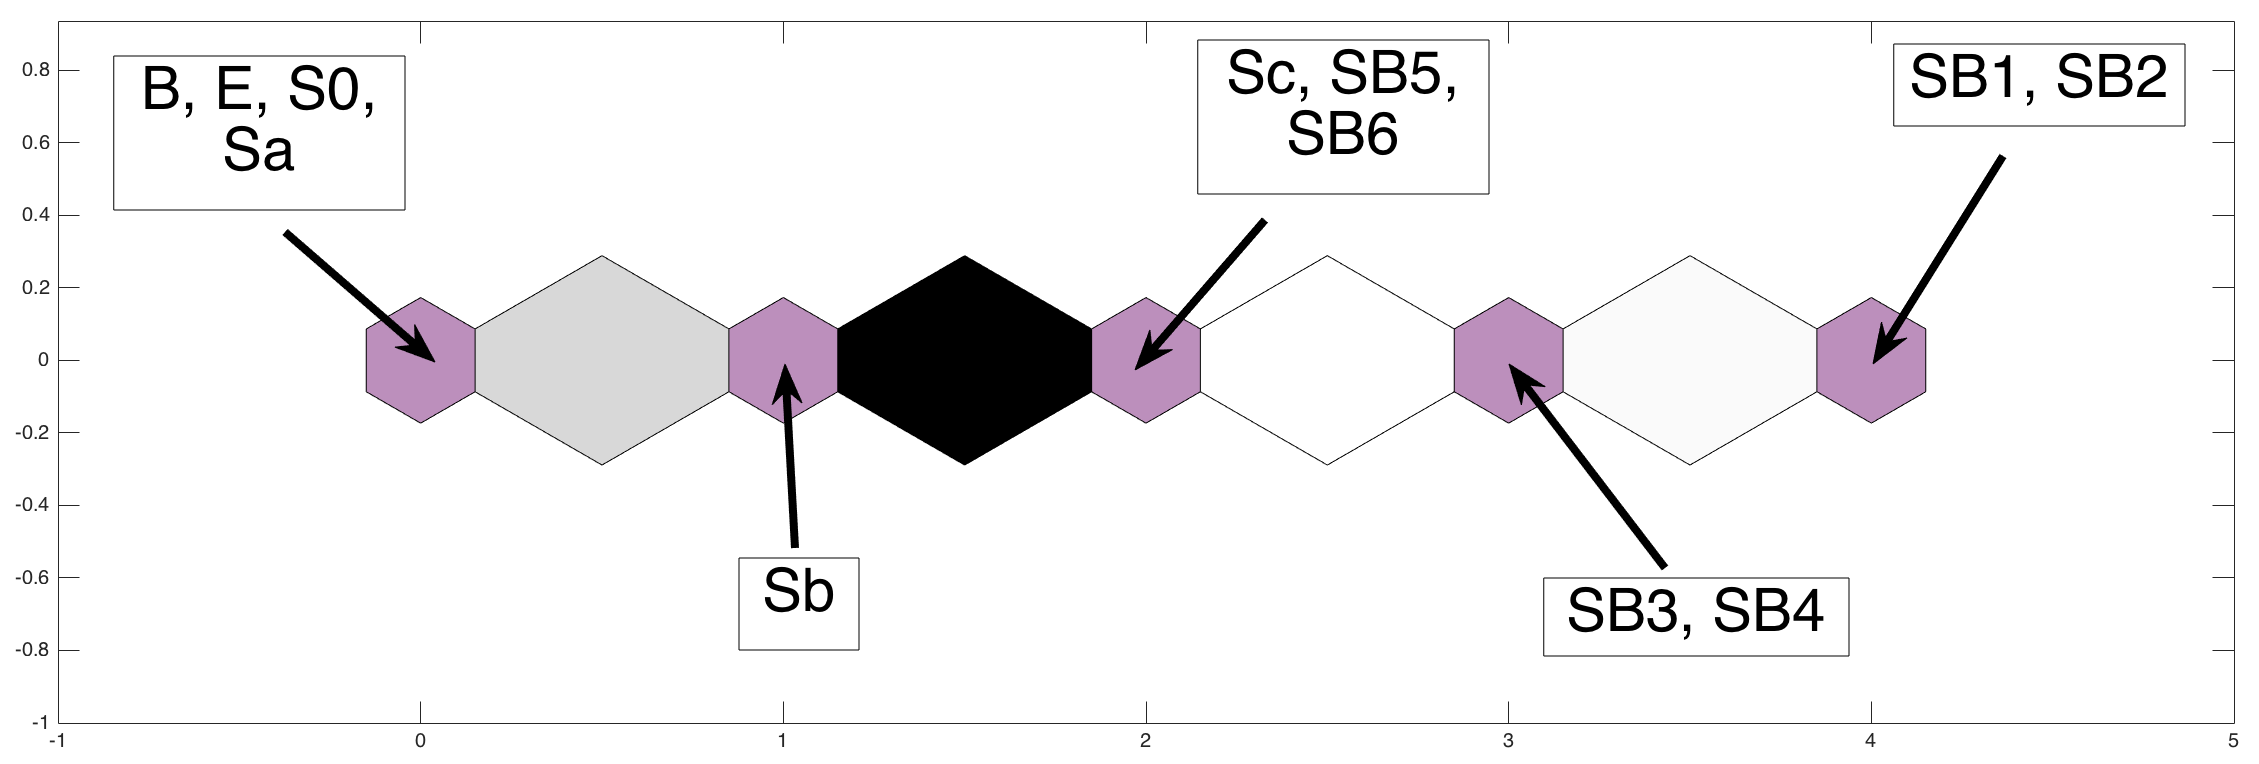
\includegraphics[width=\textwidth]{../image_paper2/1d/apps/dist_1_by_5.png}
            %\caption{$1\times5$ weight map}
             %\label{fig: 1by5T}
        \end{subfigure}
        \hfill
        \begin{subfigure}[b]{0.5\textwidth}
             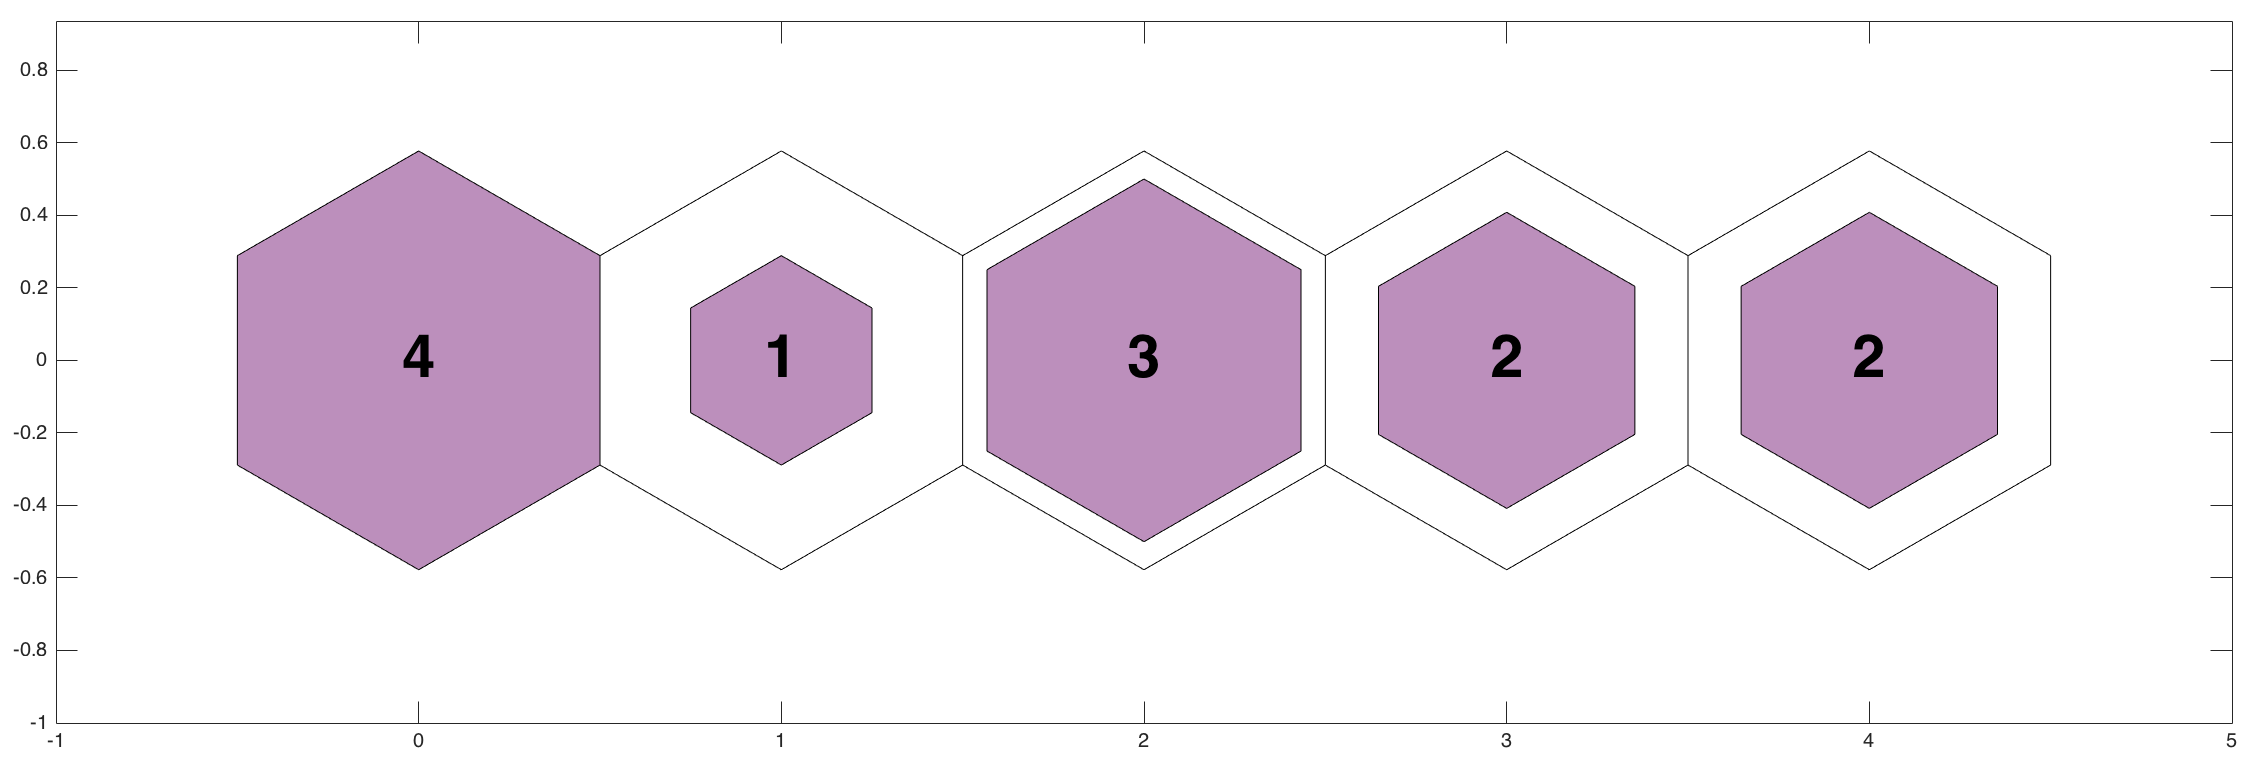
\includegraphics[width=\textwidth]{../image_paper2/1d/apps/hit_t_1_by_5.png}
             %\caption{$1\times5$ hits map}
             %\label{fig: 1by5Thits}
        \end{subfigure}
                \caption{Results of training network in $1\times5$~grid.}
         \label{fig: 1by5T}
    \end{figure}
    
    \begin{figure}
        \begin{subfigure}[b]{0.5\textwidth}
            \centering
            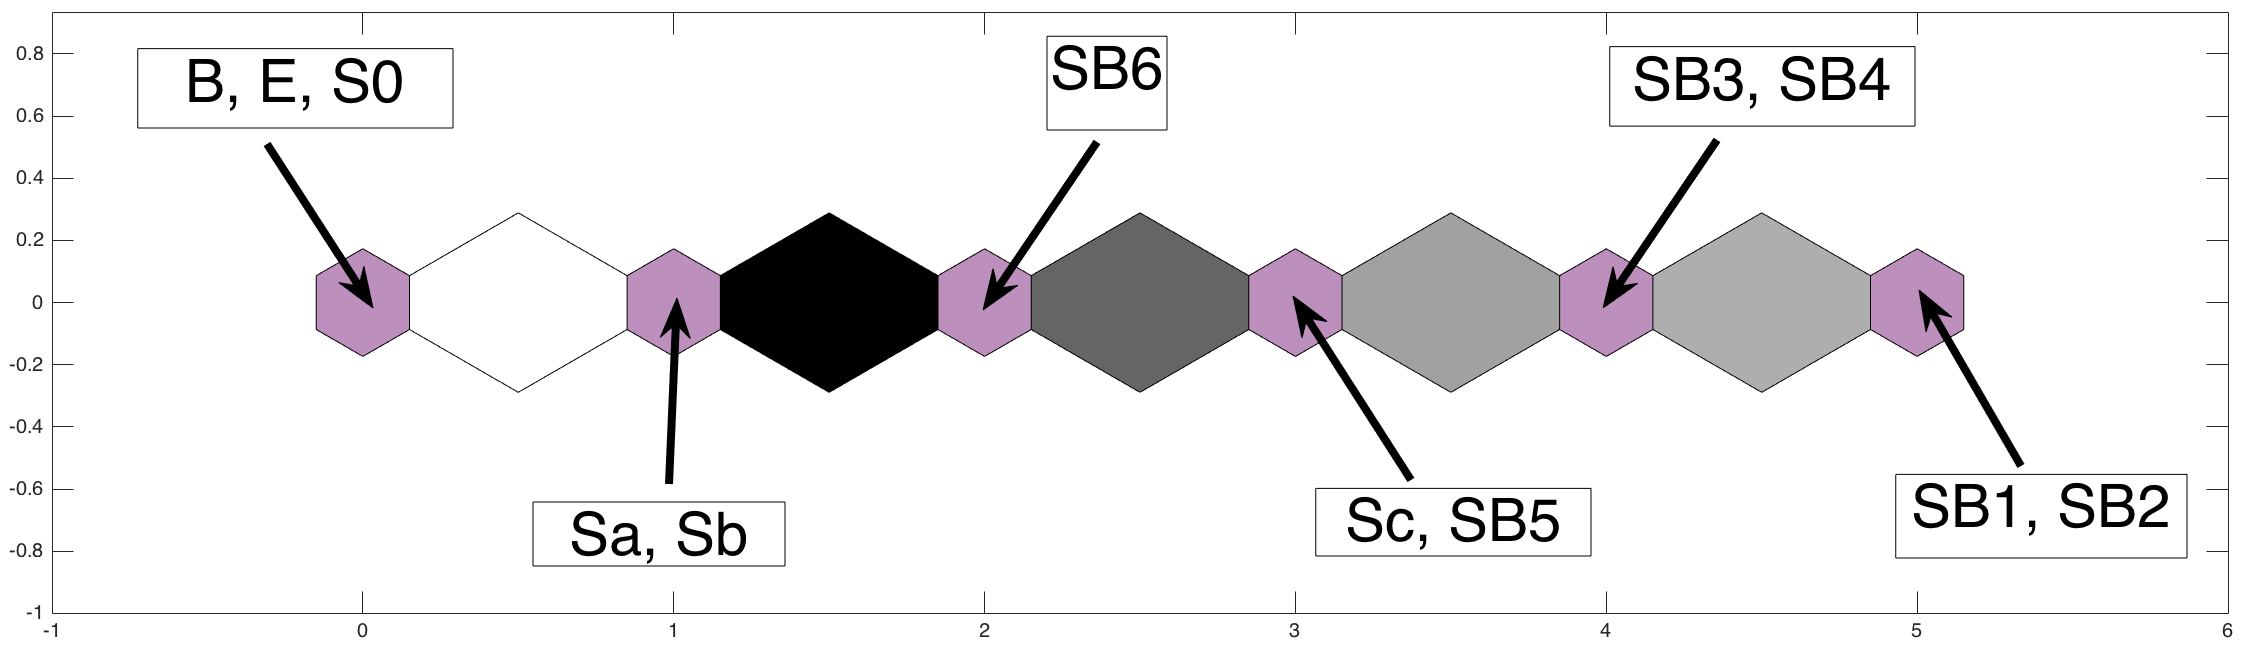
\includegraphics[width=\textwidth]{../image_paper2/1d/apps/dist_1_by_6.png}
            %\caption{$1\times6$ weight map}
             %\label{fig: 1by6T}
        \end{subfigure}
        \hfill
        \begin{subfigure}[b]{0.5\textwidth}
             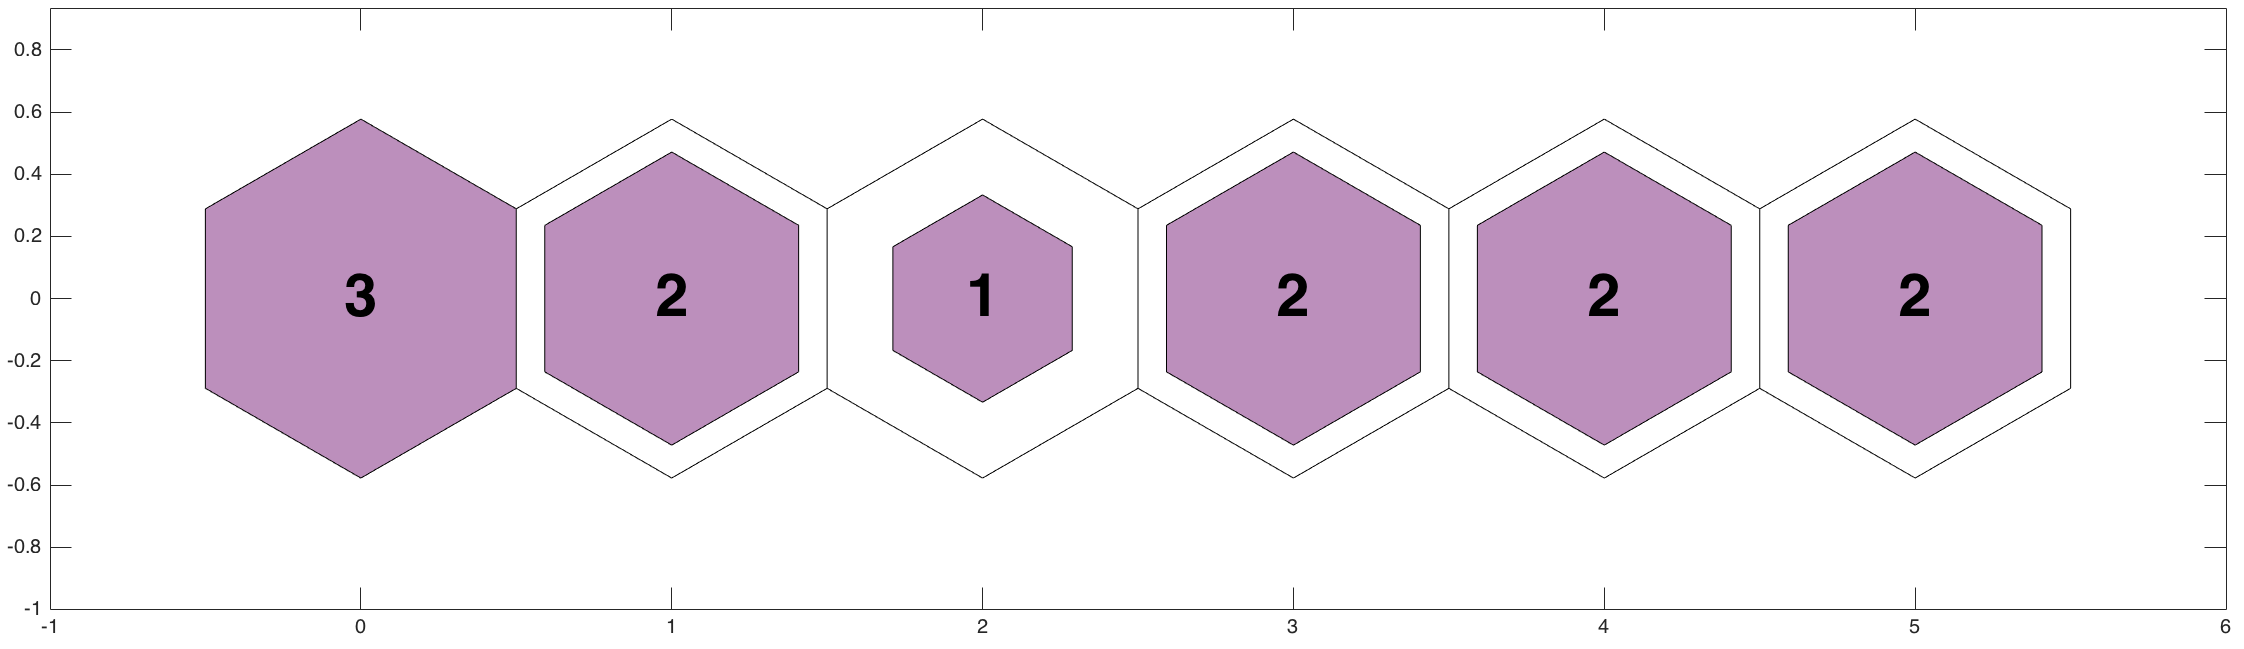
\includegraphics[width=\textwidth]{../image_paper2/1d/apps/hit_t_1_by_6.png}
             %\caption{$1\times6$ hits map}
             %\label{fig: 1by6Thits}
        \end{subfigure}
                \caption{Results of training network in $1\times6$~grid.}
         \label{fig: 1by6T}
    \end{figure}
    
    \begin{figure}
        \begin{subfigure}[b]{0.5\textwidth}
            \centering
            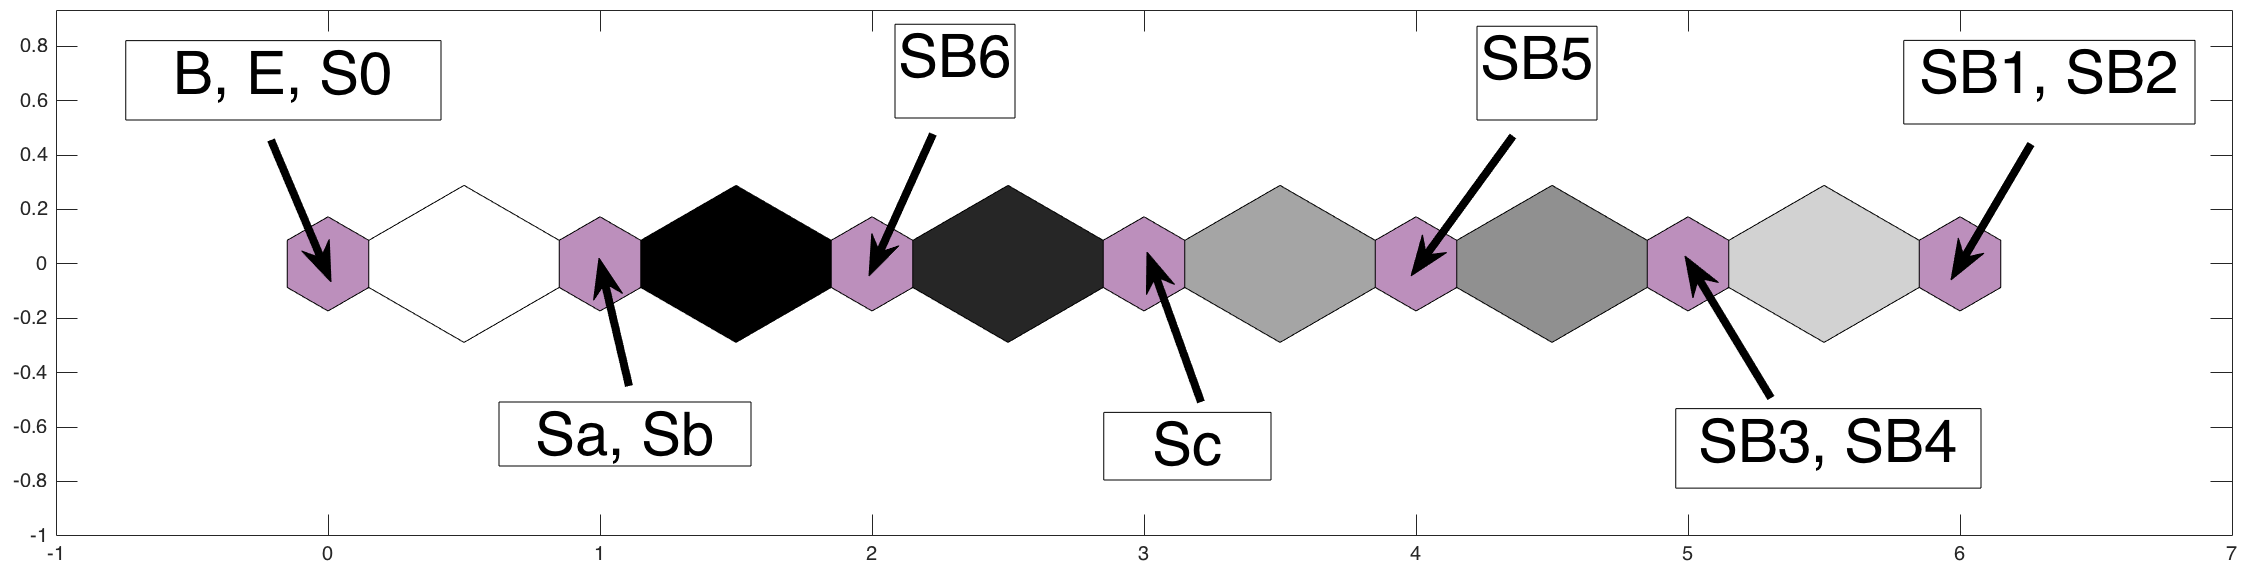
\includegraphics[width=\textwidth]{../image_paper2/1d/apps/dist_1_by_7.png}
            %\caption{$1\times7$ weight map}
             %\label{fig: 1by7T}
        \end{subfigure}
        \hfill
        \begin{subfigure}[b]{0.5\textwidth}
             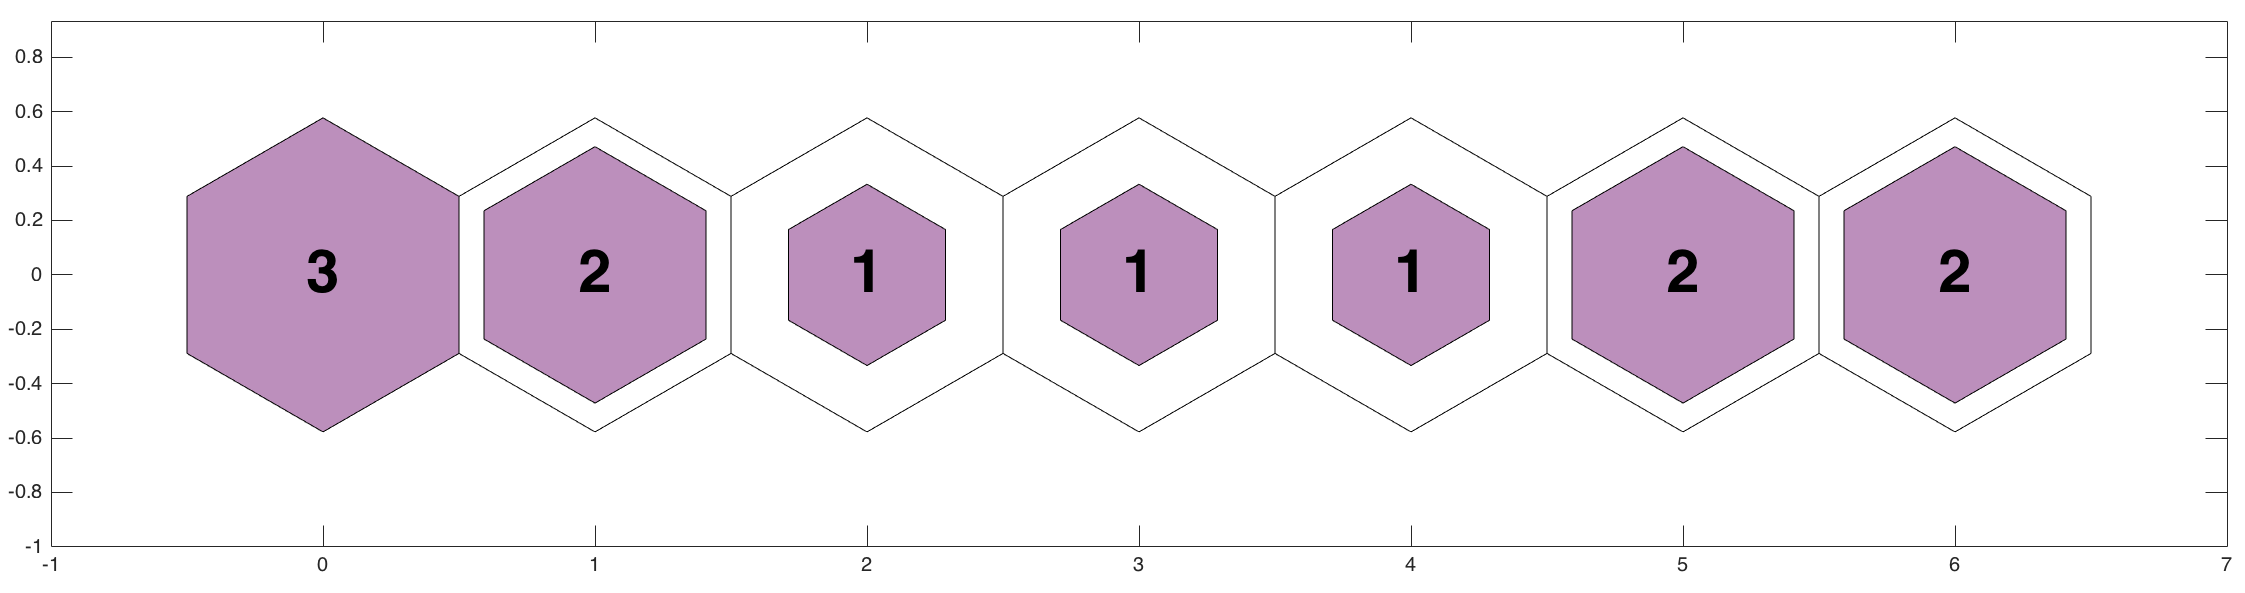
\includegraphics[width=\textwidth]{../image_paper2/1d/apps/hit_t_1_by_7.png}
             %\caption{$1\times7$ hits map}
             %\label{fig: 1by7Thits}
        \end{subfigure}
                \caption{Results of training network in $1\times7$~grid.}
         \label{fig: 1by7T}
    \end{figure}
    
    \begin{figure}
        \begin{subfigure}[b]{0.5\textwidth}
            \centering
            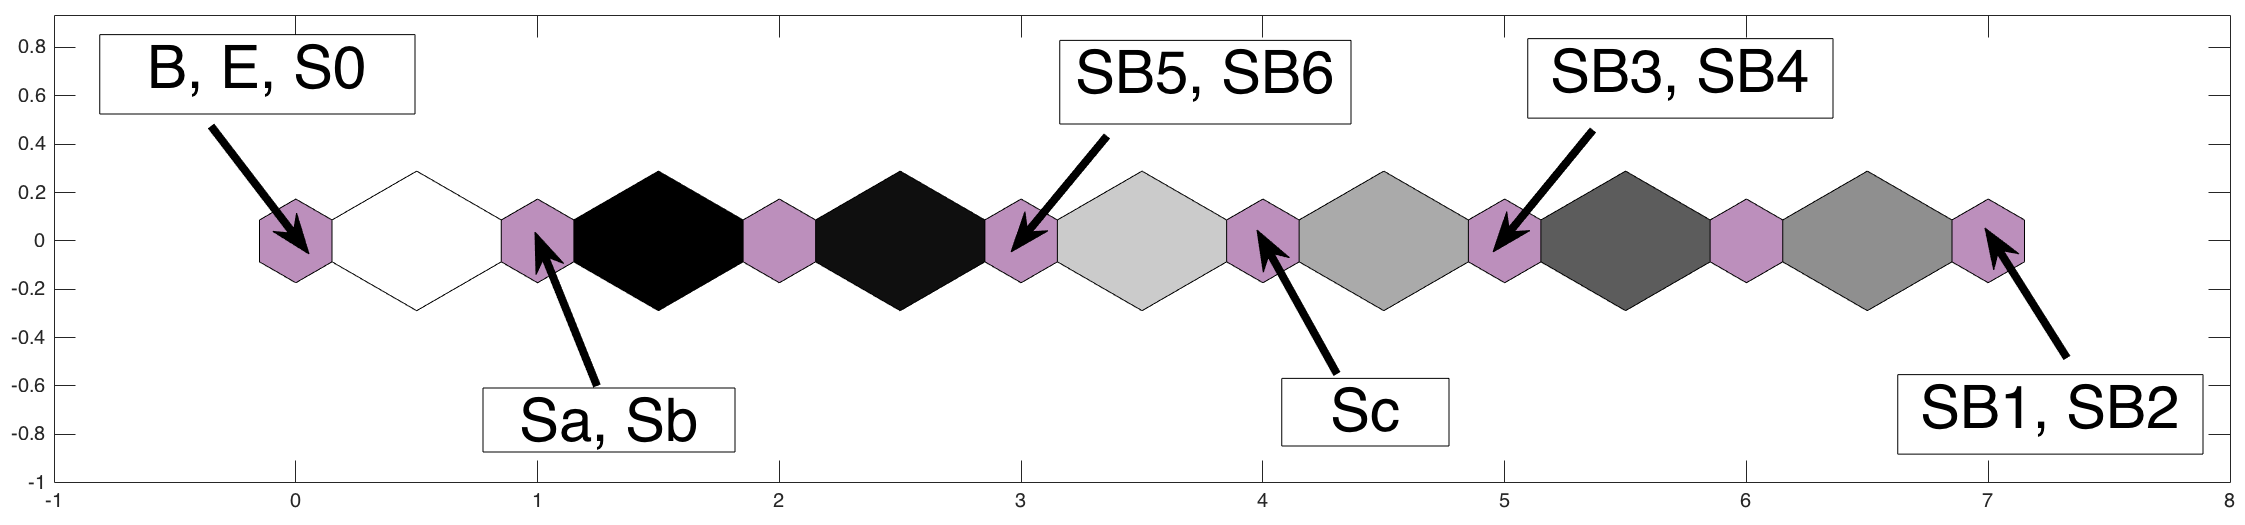
\includegraphics[width=\textwidth]{../image_paper2/1d/apps/dist_1_by_8.png}
            %\caption{$1\times8$ weight map}
             %\label{fig: 1by8T}
        \end{subfigure}
        \hfill
        \begin{subfigure}[b]{0.5\textwidth}
             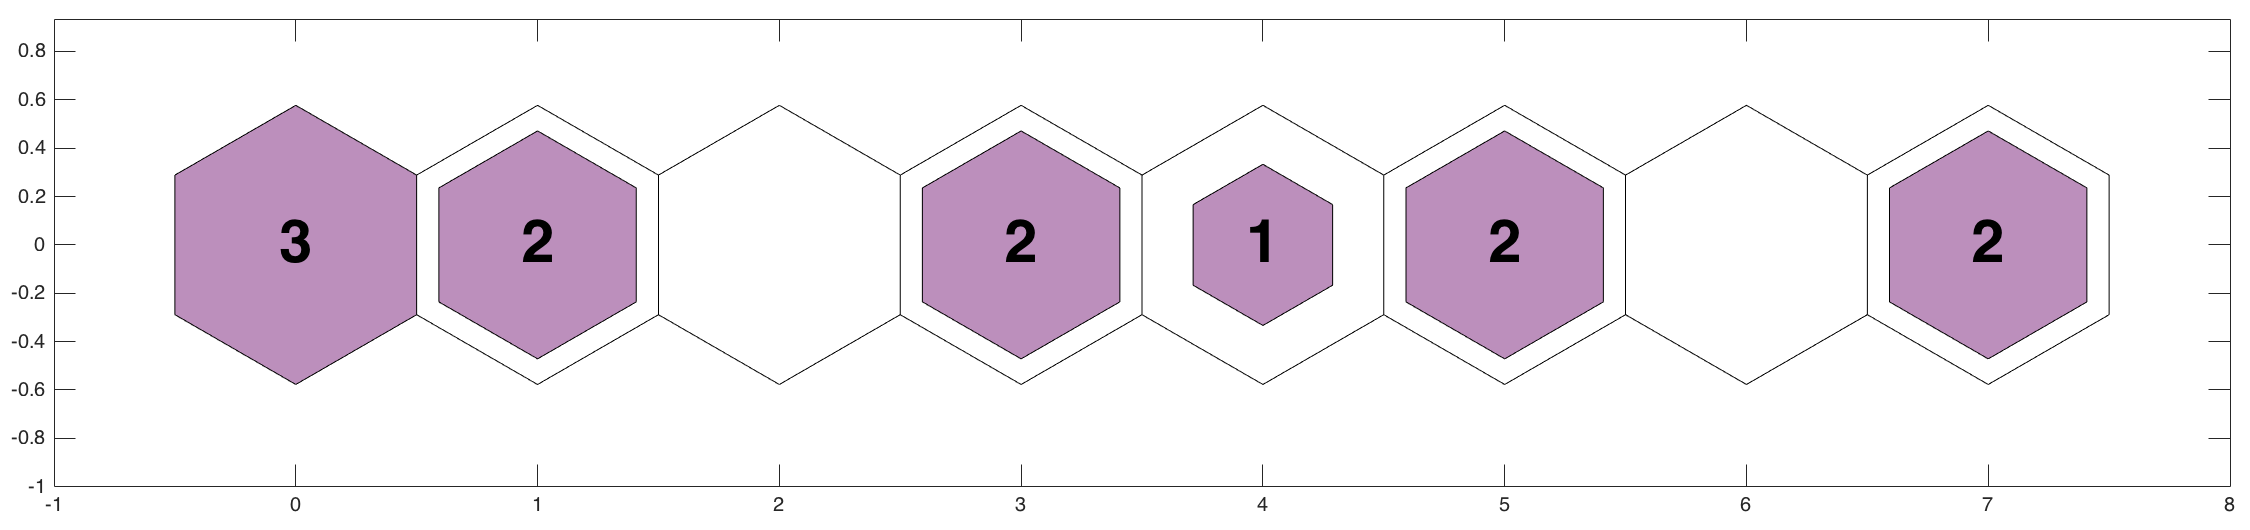
\includegraphics[width=\textwidth]{../image_paper2/1d/apps/hit_t_1_by_8.png}
             %\caption{$1\times8$ hits map}
             %\label{fig: 1by8Thits}
        \end{subfigure}
                \caption{Results of training network in $1\times8$~grid.}
         \label{fig: 1by8T}
    \end{figure}
    
    \begin{figure}
        \begin{subfigure}[b]{0.5\textwidth}
            \centering
            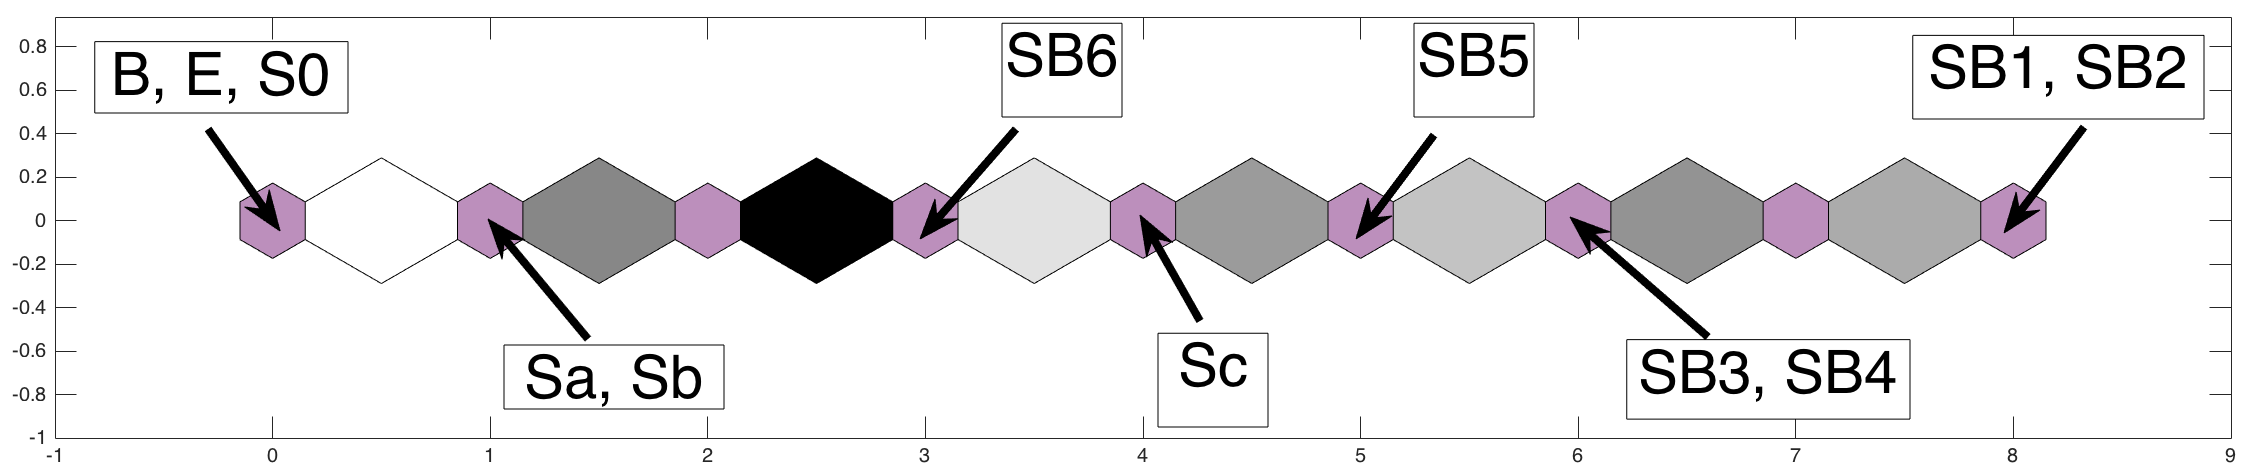
\includegraphics[width=\textwidth]{../image_paper2/1d/apps/dist_1_by_9.png}
            %\caption{$1\times9$ weight map}
             %\label{fig: 1by9T}
        \end{subfigure}
        \hfill
        \begin{subfigure}[b]{0.5\textwidth}
             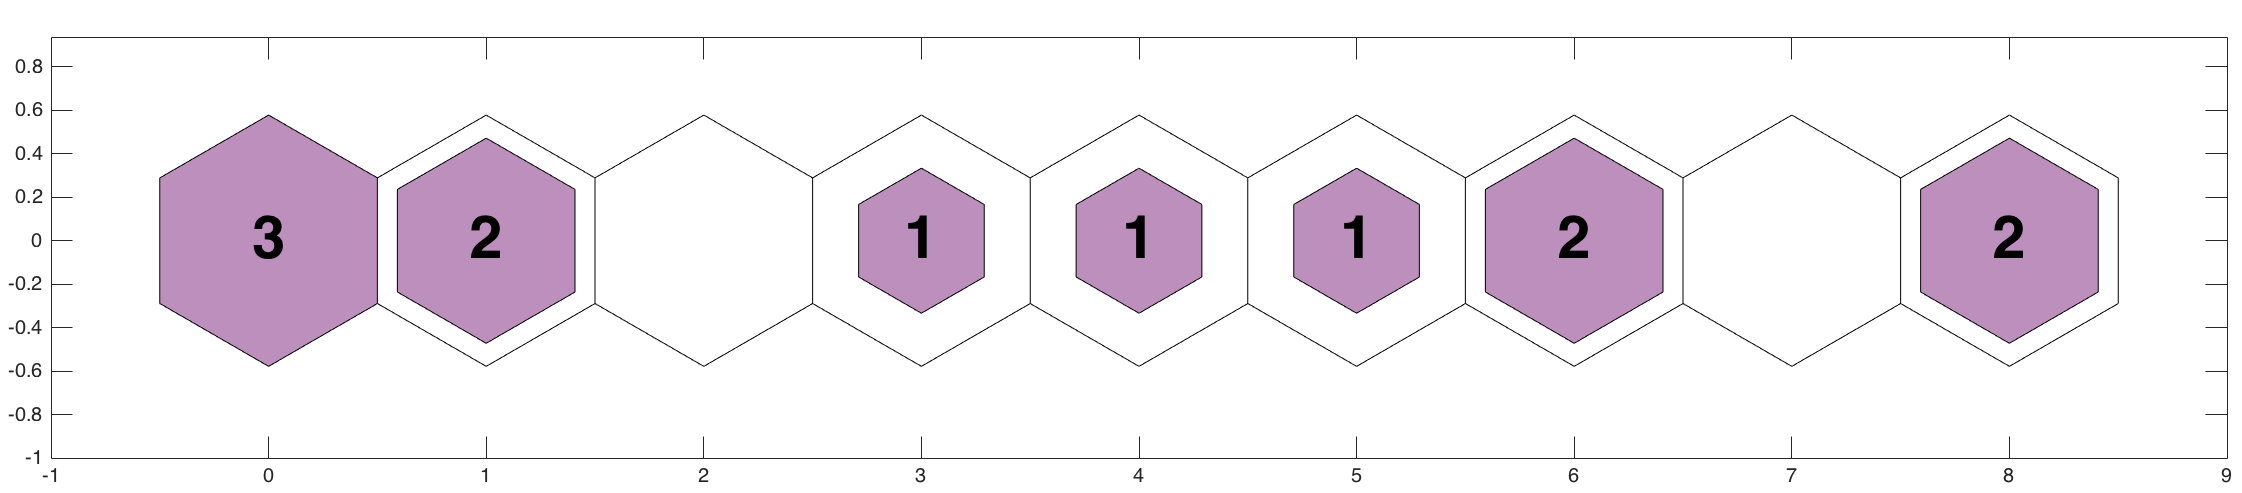
\includegraphics[width=\textwidth]{../image_paper2/1d/apps/hit_t_1_by_9.png}
             %\caption{$1\times9$ hits map}
             %\label{fig: 1by9Thits}
        \end{subfigure}
                \caption{Results of training network in $1\times9$~grid.}
         \label{fig: 1by9T}
    \end{figure}

    \begin{figure}
        \begin{subfigure}[b]{0.5\textwidth}
            \centering
            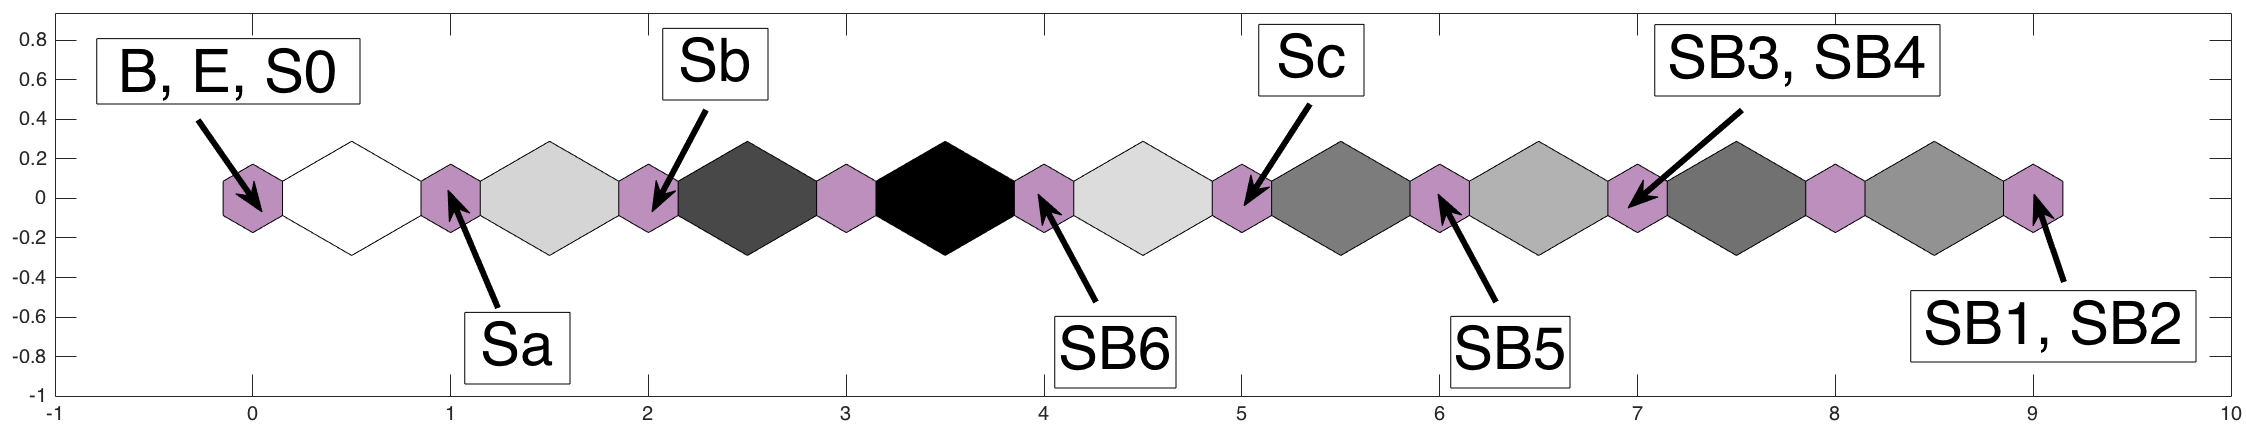
\includegraphics[width=\textwidth,height=2.5cm]{../image_paper2/1d/apps/dist_1_by_10.png}
            %\caption{$1\times10$ weight map}
             %\label{fig: 1by10T}
        \end{subfigure}
        \hfill
        \begin{subfigure}[b]{0.5\textwidth}
             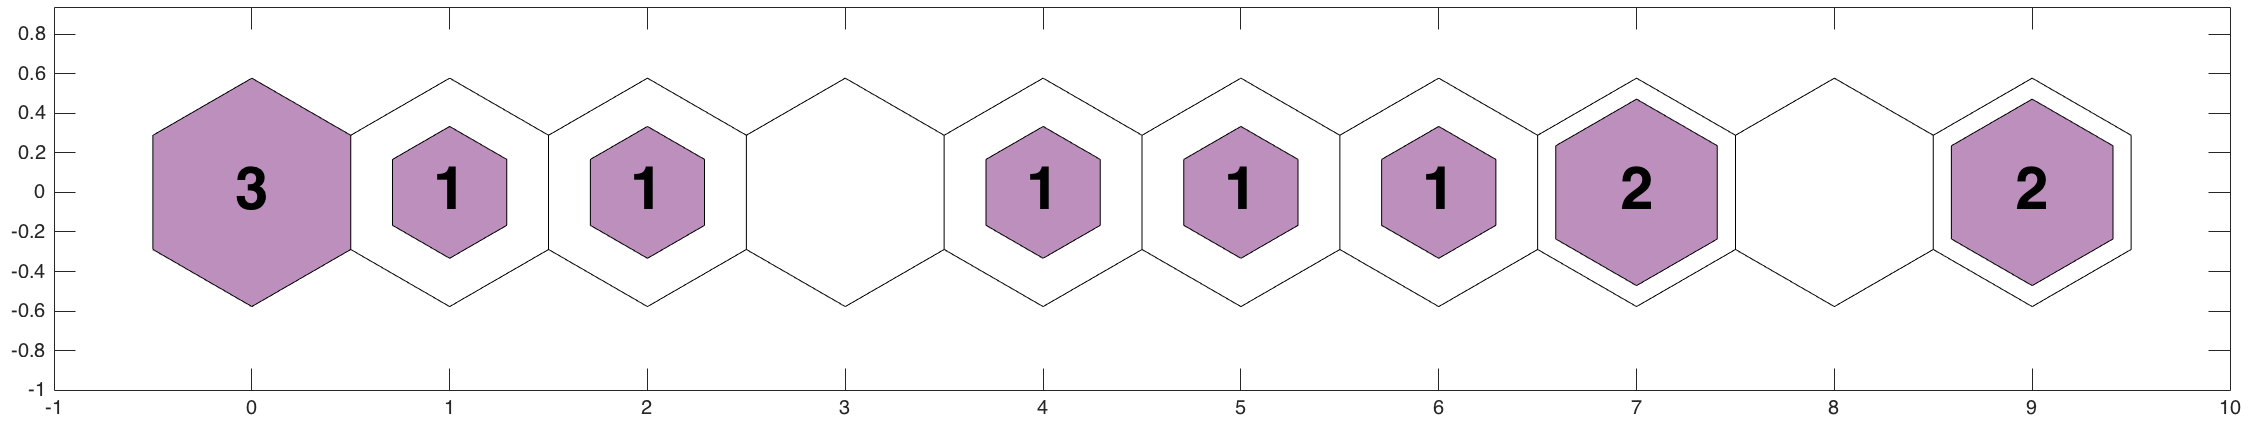
\includegraphics[width=\textwidth,height=2.5cm]{../image_paper2/1d/apps/hit_t_1_by_10.png}
             %\caption{$1\times10$ hits map}
             %\label{fig: 1by10Thits}
        \end{subfigure}
                \caption{Results of training network in $1\times10$~grid.}
         \label{fig: 1by10T}
    \end{figure}

    \begin{figure}
        \begin{subfigure}[b]{0.5\textwidth}
            \centering
            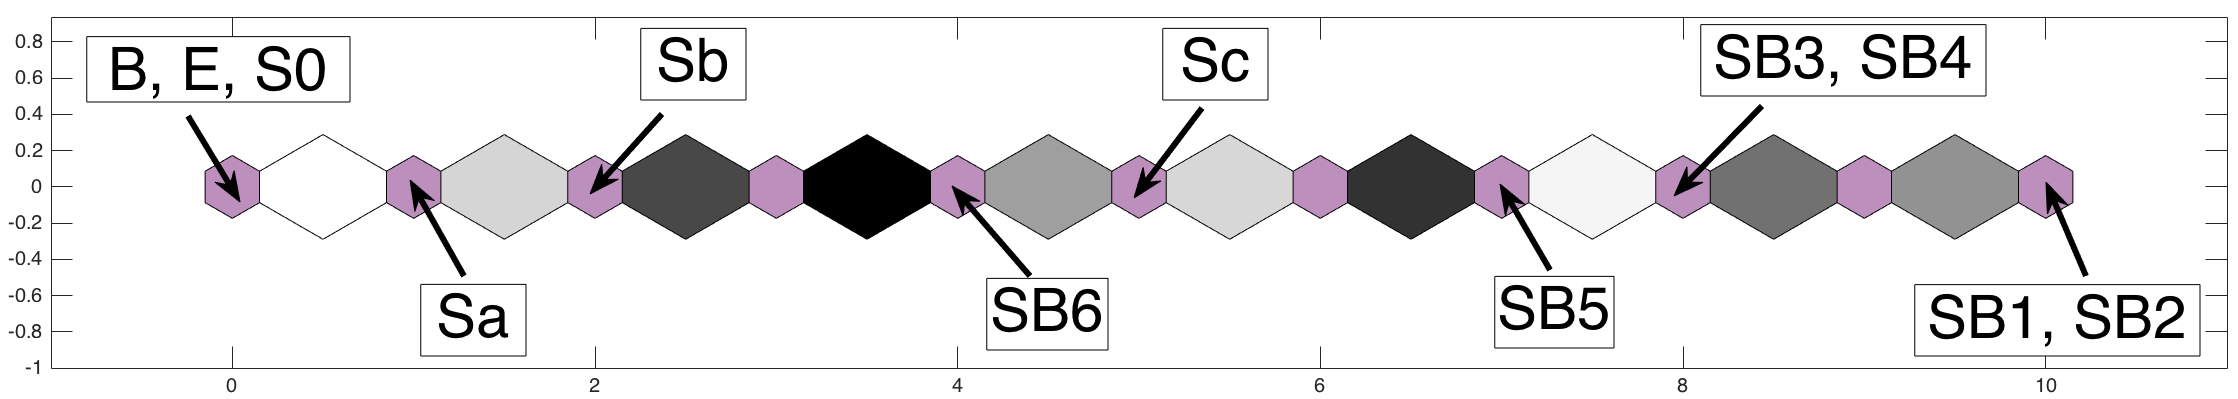
\includegraphics[width=\textwidth,height=2.5cm]{../image_paper2/1d/apps/dist_1_by_11.png}
            %\caption{$1\times11$ weight map}
             %\label{fig: 1by11T}
        \end{subfigure}
        \hfill
        \begin{subfigure}[b]{0.5\textwidth}
             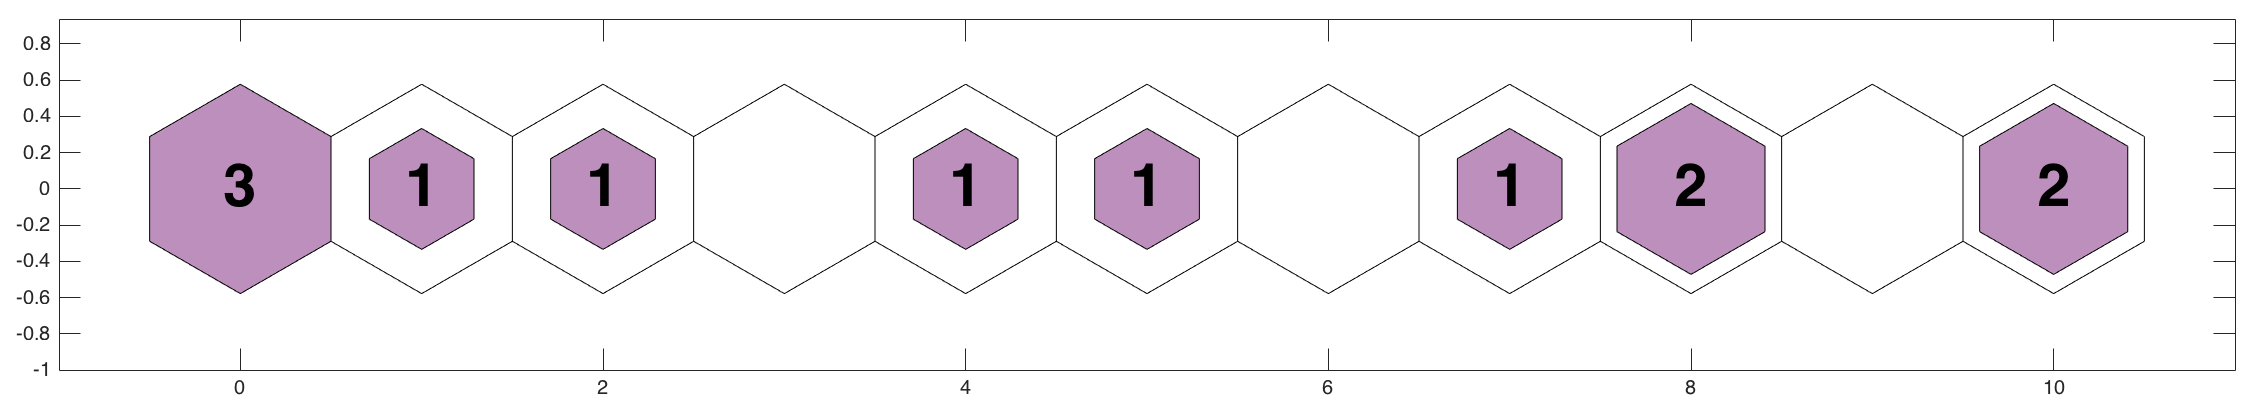
\includegraphics[width=\textwidth,height=2.5cm]{../image_paper2/1d/apps/hit_t_1_by_11.png}
             %\caption{$1\times11$ hits map}
             %\label{fig: 1by11Thits}
        \end{subfigure}
                \caption{Results of training network in $1\times11$~grid.}
         \label{fig: 1by11T}
    \end{figure}
    

    \begin{figure}
        \begin{subfigure}[b]{0.5\textwidth}
            \centering
            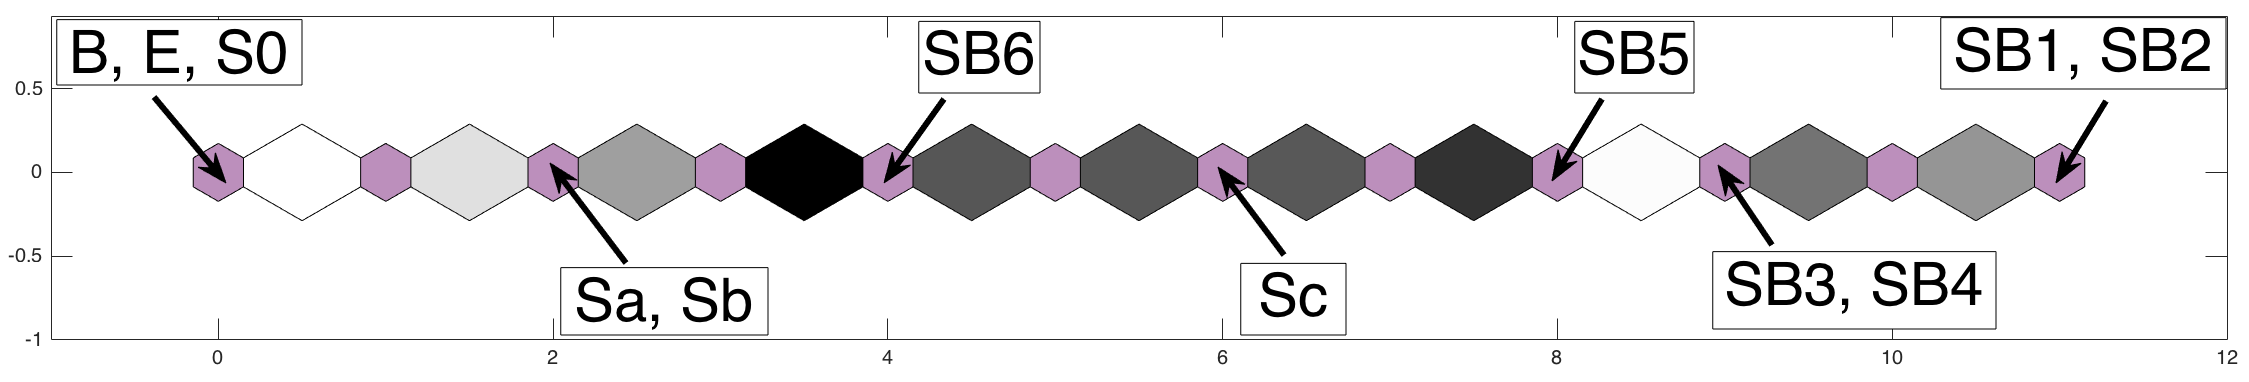
\includegraphics[width=\textwidth,height=2.5cm]{../image_paper2/1d/apps/dist_1_by_12.png}
            %\caption{$1\times12$ weight map}
             %\label{fig: 1by12T}
        \end{subfigure}
        \hfill
        \begin{subfigure}[b]{0.5\textwidth}
             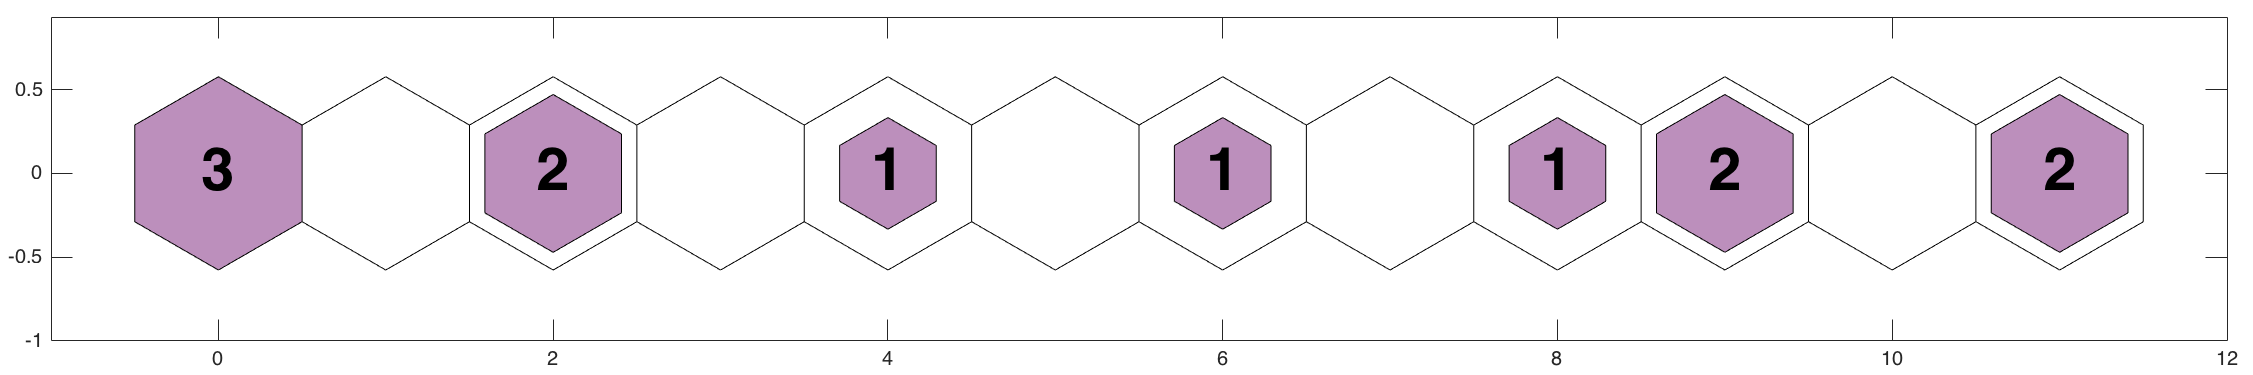
\includegraphics[width=\textwidth,height=2.5cm]{../image_paper2/1d/apps/hit_t_1_by_12.png}
             %\caption{$1\times12$ hits map}
             %\label{fig: 1by12Thits}
        \end{subfigure}
                \caption{Results of training network in $1\times12$~grid.}
         \label{fig: 1by12T}
    \end{figure}

    \begin{figure}
        \begin{subfigure}[b]{0.5\textwidth}
            \centering
            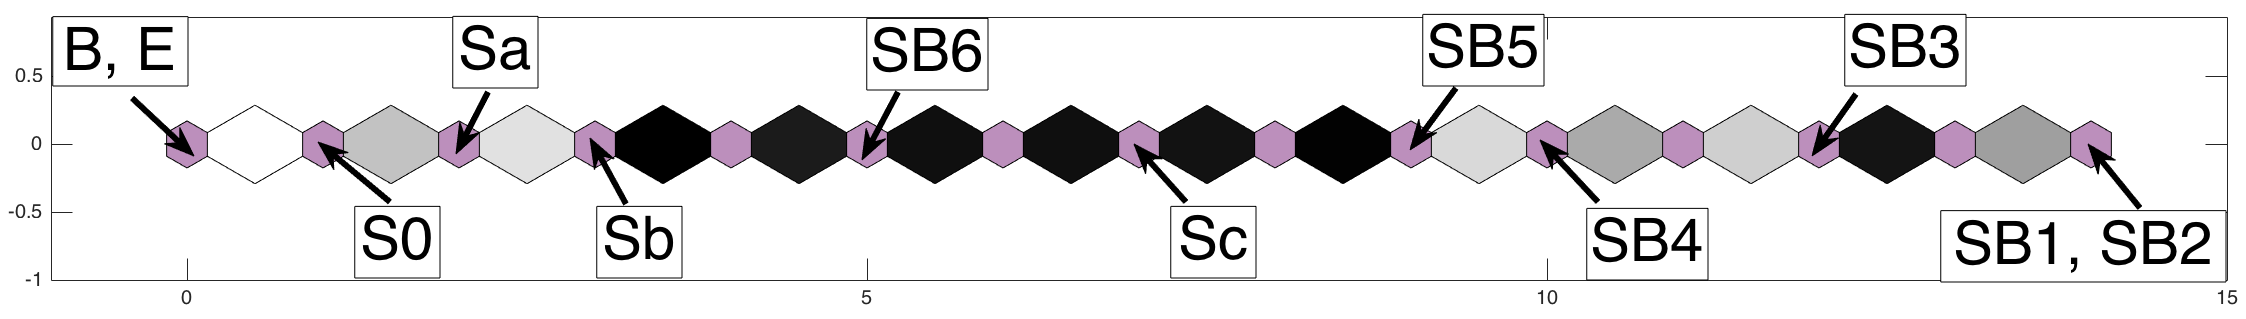
\includegraphics[width=\textwidth,height=2.5cm]{../image_paper2/1d/apps/dist_1_by_15.png}
            %\caption{$1\times15$ weight map}
             %\label{fig: 1by15T}
        \end{subfigure}
        \hfill
        \begin{subfigure}[b]{0.5\textwidth}
             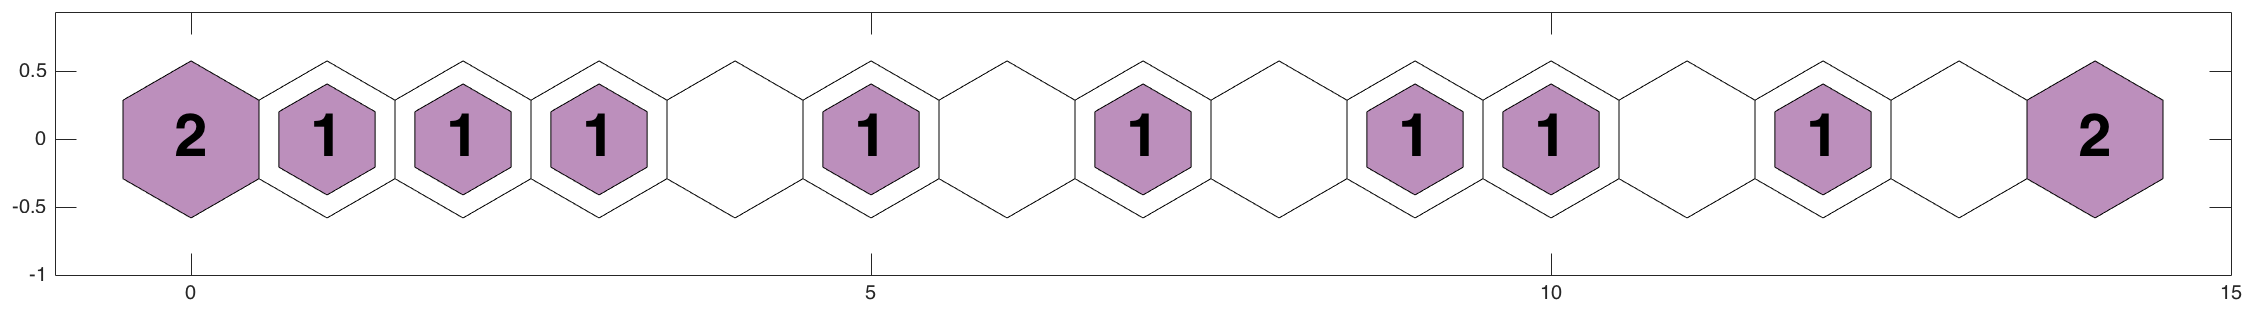
\includegraphics[width=\textwidth,height=2.5cm]{../image_paper2/1d/apps/hit_t_1_by_15.png}
             %\caption{$1\times15$ hits map}
             %\label{fig: 1by15Thits}
        \end{subfigure}
                \caption{Results of training network in $1\times15$~grid.}
         \label{fig: 1by15T}
    \end{figure}

    \begin{figure}
        \begin{subfigure}[b]{0.5\textwidth}
            \centering
            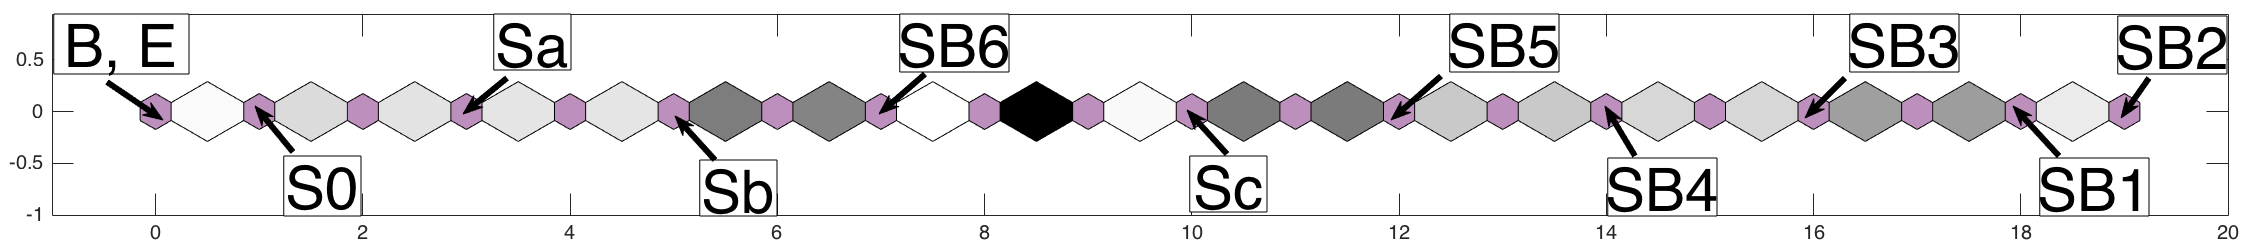
\includegraphics[width=\textwidth,height=2.5cm]{../image_paper2/1d/apps/dist_1_by_20.png}
            %\caption{$1\times20$ weight map}
             %\label{fig: 1by20T}
        \end{subfigure}
        \hfill
        \begin{subfigure}[b]{0.5\textwidth}
             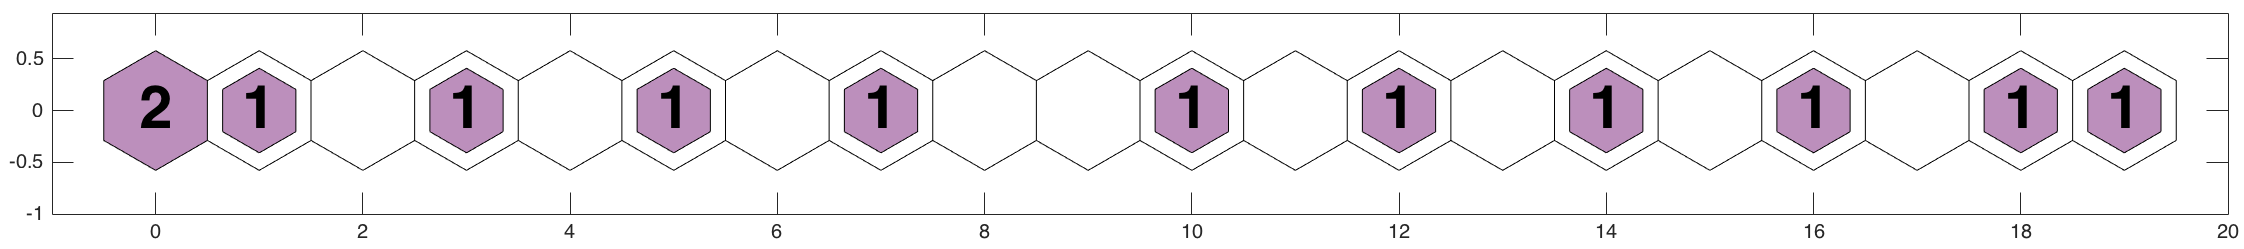
\includegraphics[width=\textwidth,height=2.5cm]{../image_paper2/1d/apps/hit_t_1_by_20.png}
             %\caption{$1\times20$ hits map}
             %\label{fig: 1by20Thits}
        \end{subfigure}
                \caption{Results of training network in $1\times20$~grid.}
         \label{fig: 1by20T}
    \end{figure}
    
